\documentclass[a4paper,11pt]{article}
\usepackage{graphicx}
\usepackage{amsmath}
\usepackage{amssymb}
\usepackage{fancyhdr}
\usepackage{lipsum}
\usepackage{pdfpages}

\pagestyle{fancy}
\fancyhead[L]{Kuldeep1709}
\fancyhead[C]{Linear Algebra-18.06 MIT 2005}
\fancyhead[R]{Gilbert Strang}

\numberwithin{equation}{section}
\begin{document}
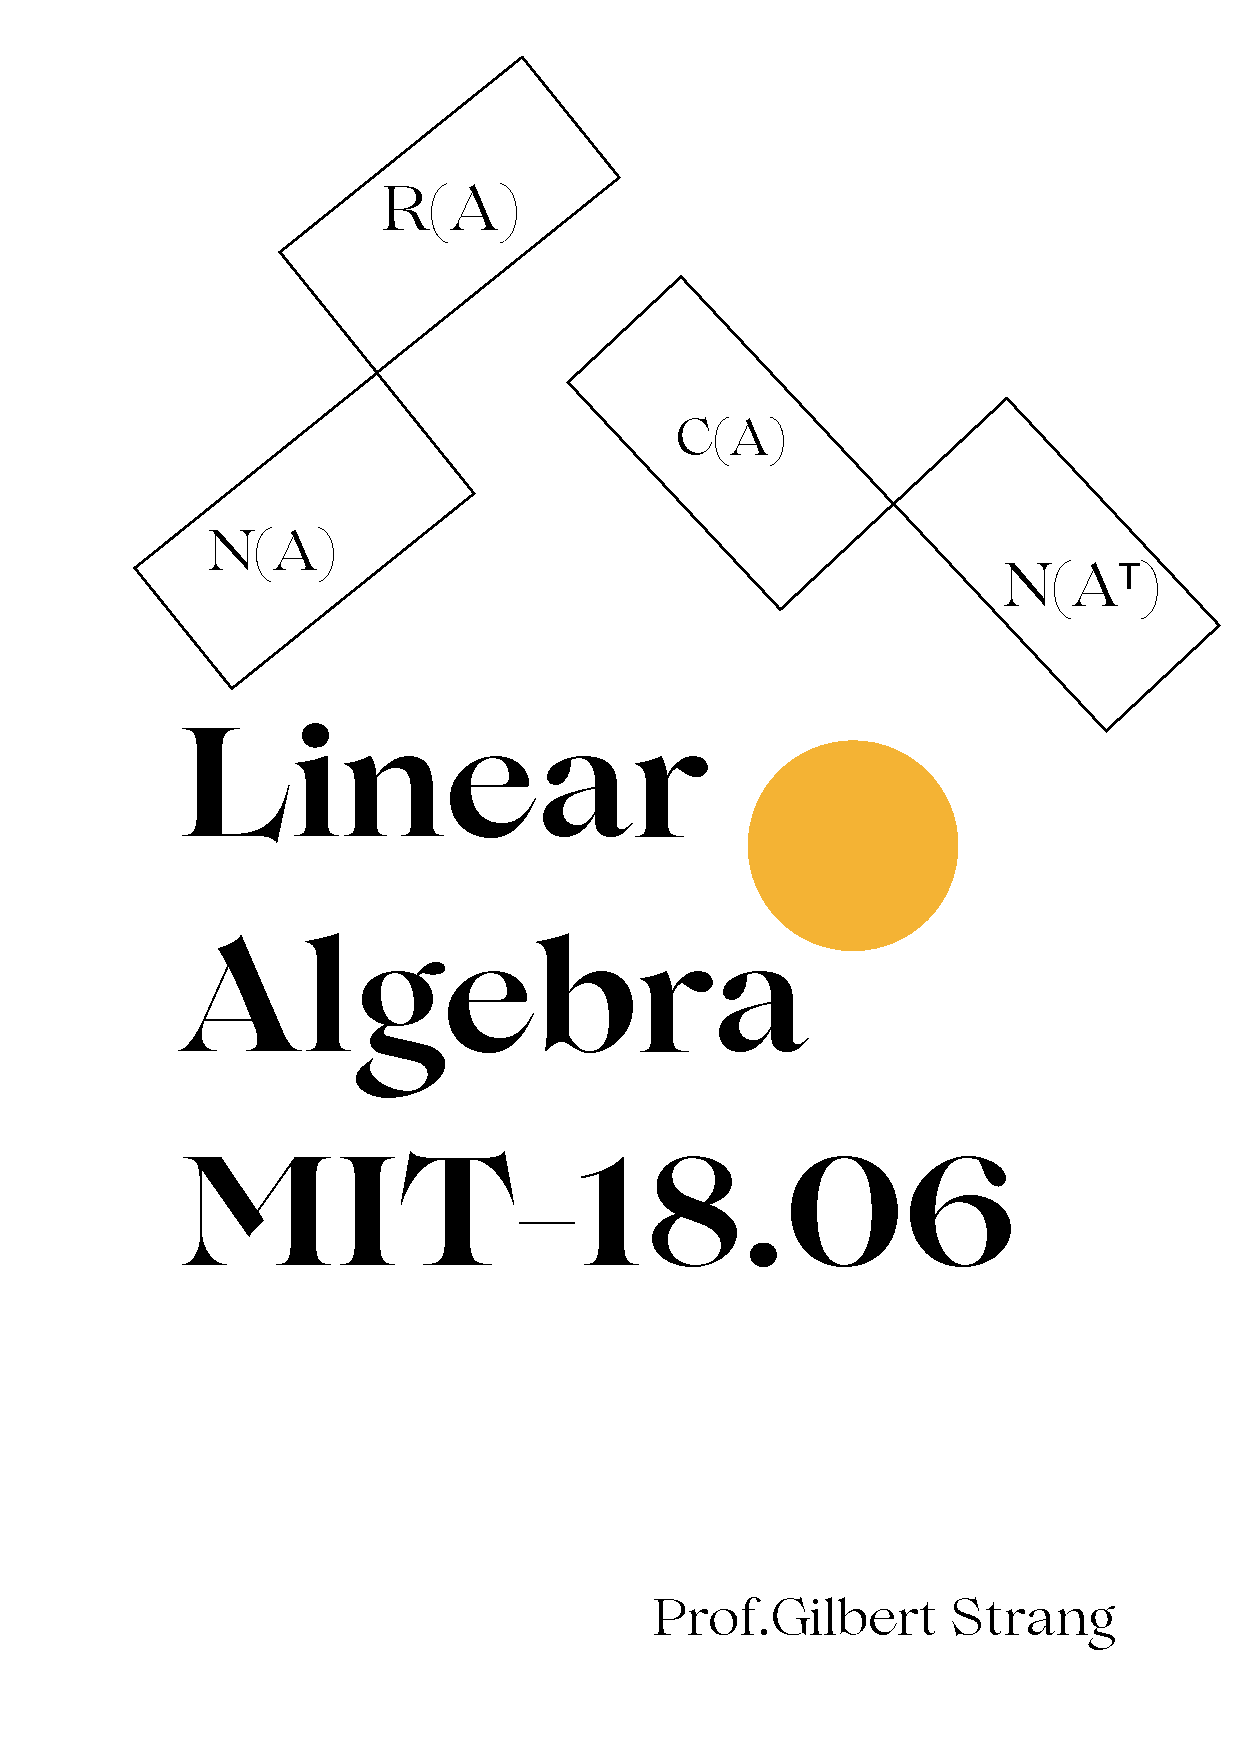
\includepdf[pages=1,fitpaper]{FrontPage}

    \begin{center}
        \Huge{\textbf{Lecture-1}}
    \end{center}
    \vspace{5pt}
    \begin{itemize}
        \item \textbf{System of Linear Equations}
            \vspace{5pt}\\
            Given n linear equations n variables can be represented in the form of matrices and there multiplication.\\
            \vspace{5pt} 
            \begin{center}
                $a_{12}x_{1}+a_{12}x_2\dots +a_{1n}x_n=b1$\\
                $a_{21}x_{1}+a_{22}x_2\dots +a_{2n}x_n=b2$\\
                $\vdots$\\
                $a_{n1}x_{1}+a_{n2}x_2\dots +a_{nn}x_n=bn$\\

                \vspace{4pt}
                these above equations can be written a

            \end{center}
            \begin{center}
                $Ax=b$
            \end{center}
            where A is a matrix of coefficients of variables and b is a matrix of constants.\\
            \begin{equation}
                \begin{bmatrix}
                    a_{11} & a_{12} & a_{13} & \cdots & a_{1n} \\
                    a_{21} & a_{22} & a_{23} & \cdots & a_{2n} \\
                    \vdots & \vdots & \vdots & \ddots & \vdots \\
                    a_{n1} & a_{n2} & a_{n3} & \cdots & a_{nn} \\
                \end{bmatrix}
                \begin{bmatrix}
                    x_{1} \\
                    x_{2} \\
                    \vdots \\
                    x_{n} \\
                \end{bmatrix}
                =
                \begin{bmatrix}
                    b_{1} \\
                    b_{2} \\
                    \vdots \\
                    b_{n} \\
                \end{bmatrix}
            \end{equation}
        \vspace{5pt}
        \item \textbf{How to Look at Matrices}
            \vspace{5pt}\\
            Let's have a System of linear equations.\\
            % \vspace{3pt}
            \begin{center}
                $2x-y=0$\\
                $-x+2y=3$\\
            \end{center}
            \begin{itemize}
                \item \textbf{Row Picture}
                    \vspace{5pt}
                    \begin{center}
                        $Ax=b$
                    \end{center}
                            \[\begin{bmatrix}
                                2 & -1 \\
                                -1 & 2 \\
                            \end{bmatrix}
                            \begin{pmatrix}
                                x\\
                                y\\
                            \end{pmatrix}=
                            \begin{pmatrix}
                                0\\
                                3\\
                            \end{pmatrix}
                            \]                
                \item \textbf{Column Picture}
                    \vspace{5pt}\\
                    Here we scaling column vectors by x \& y and trying to get the resultant vector as b.\\
                    \begin{center}
                        $Ax=b$
                    \end{center}
                            \[x
                            \begin{pmatrix}
                                2  \\
                                -1  \\
                            \end{pmatrix}+y
                            \begin{pmatrix}
                                -1\\
                                2\\
                            \end{pmatrix}=
                            \begin{pmatrix}
                                0\\
                                3\\
                            \end{pmatrix}
                            \]
            \end{itemize}
        \item \textbf{Que:} Can we Get any vector by just scaling column vectors \textbf{?}
        \item \textbf{Ans:} Well it depends on the column vectors or column space. If the column vectors are linearly independent or $\vec{b}$ is in column space then we can get any vector by scaling them! \\$ref. Lecture 6!$\\
    \item \textbf{Multiplying a matrix with a vector}\\
    
    \vspace{5pt}
    
        \begin{itemize}
            \item \textbf{Row-Column Way:}\\
                \begin{equation}
                    \begin{bmatrix}
                        a & b \\
                        c & d \\
                    \end{bmatrix}
                    \begin{bmatrix}
                        x \\
                        y \\
                    \end{bmatrix}
                    =
                    \begin{bmatrix}
                        ax+by \\
                        cx+dy \\
                    \end{bmatrix}
                \end{equation}
            \item \textbf{Column-Row Way:}\\
                \begin{equation}
                    \begin{bmatrix}
                        a & b \\
                        c & d \\
                    \end{bmatrix}
                    \begin{bmatrix}
                        x \\
                        y \\
                    \end{bmatrix}
                    =
                        x
                        \begin{bmatrix}
                            a \\
                            c \\
                        \end{bmatrix}
                        +y
                        \begin{bmatrix}
                            b \\
                            d \\
                        \end{bmatrix}
                \end{equation}\\
            Means the Transformation vector of 
            \[
                \begin{pmatrix}
                    x \\
                    y \\
                \end{pmatrix}
            \] 
            is x times the column 1 and y times the column 2.
        \end{itemize}
    \end{itemize}
    \vspace{1cm}
    \begin{center}
        \Huge{\textbf{Lecture-2}}
    \end{center}
    \vspace{5pt}
    \begin{itemize}         
        \item \textbf{Solving Linear Equations : Ellimination}\\
        Let us have this system of linear equations to solve
        \begin{center}
            $x+2y+z=1$\\
            $3x+8y+z=1$\\
            $4y+z=1$\\
        \end{center}

        then corrsoponding to this system of linear equations we have a matrix equation as.

        \begin{equation}
            \begin{bmatrix}
                1 & 2 & 1 \\
                3 & 8 & 1 \\
                0 & 4 & 1 \\
            \end{bmatrix}
            \begin{pmatrix}
                x \\
                y \\
                z \\
            \end{pmatrix}=
            \begin{pmatrix}
                2 \\
                12 \\
                2 \\
            \end{pmatrix}
        \end{equation}
        \begin{itemize}
            \item \textbf{Step I: Ellimination}\\
            \begin{itemize}
                \item \textbf{Step-1:} Subtract 3 times the first row from the second row.
                \begin{equation}
                    \begin{bmatrix}
                        1 & 2 & 1 \\
                        0 & 2 & -2 \\
                        0 & 4 & 1 \\
                    \end{bmatrix}
                    \begin{pmatrix}
                        x \\
                        y \\
                        z \\
                    \end{pmatrix}=
                    \begin{pmatrix}
                        2 \\
                        6 \\
                        2 \\
                    \end{pmatrix}
                \end{equation}
                \item \textbf{Step-2:} Subtract 2 times the second row from the third row.
                \begin{equation}
                    \begin{bmatrix}
                        1 & 2 & 1 \\
                        0 & 2 & -2 \\
                        0 & 0 & 5 \\
                    \end{bmatrix}
                    \begin{pmatrix}
                        x \\
                        y \\
                        z \\
                    \end{pmatrix}=
                    \begin{pmatrix}
                        2 \\
                        6 \\
                        10 \\
                    \end{pmatrix}
                \end{equation}
            \end{itemize}

        \item \textbf{Step II : Back Substitution}\\
            Cleary now if convert this into Linear equations
            we will get\\

            \begin{center}
                $x+2y+z=2$\\
                $2y-2z=6$\\
                $5z=10$\\
            \end{center}

            So, $z=2,y=5,x=-12$ is the Solution to the Linear Equations.        
        \end{itemize}
       

        \item \textbf{Validity of Ellimination : }Note that Ellimination method will be able to solve the system of  linear equations iff the coefficient matrix is \textbf{Invertible} (Ref. Next Lecture Notes).\\
        In case if the coefficient matrix is Invertible then our Ellimination method will encounter \textbf{Pivots} as $0$ in the process. but those will be handled using row Exchanges.

        \item \textbf{Ellimination Matrices}
        \vspace{5pt}\\
        Above in step \textbf{I.1} and \textbf{I.2} we did row operations and finally arrived at the solution.Those elliminations can be expressed in the from other matrices for example\\
        \begin{equation}
            Elemenation^1=E_1=
            \begin{bmatrix}
                1 & 2 & 1 \\
                0 & 2 & -2 \\
                0 & 4 & 1 \\
            \end{bmatrix}=
            \begin{bmatrix}
                1 & 0 & 0 \\
                -3 & 1 & 0 \\
                0 & 0 & 1 \\
            \end{bmatrix} \times A
        \end{equation}

        and then \\
        \begin{equation}
            Elemenation^2=
            \begin{bmatrix}
                1 & 2 & 1 \\
                0 & 2 & -2 \\
                0 & 0 & 5 \\
            \end{bmatrix}=
            \begin{bmatrix}
                1 & 0 & 0 \\
                0 & 1 & 0 \\
                0 & -2 & 1 \\
            \end{bmatrix} \times E_1
        \end{equation}

        \begin{equation}
            Final Matrix=
            \begin{bmatrix}
                1 & 2 & 1 \\
                0 & 2 & -2 \\
                0 & 0 & 5 \\
            \end{bmatrix}=
            (E_1 \times E_2) \times A
        \end{equation}

        \begin{center}
            Let,      $E=E_1 \times E_2$
        \end{center}

        So the whole elemenation process can be just reduced to this Matrix \textbf{$E$} known as \textbf{Ellimination Matrix.}

        \item \textbf{How to find these elemenation matrices? is there any method??}

        \item \textbf{Yes: Realzation of Left \& Right Matrix Multiplication}\\
            Starting with a matrix with column and then a row with matrix Multiplication.Given matrices $A$ \& $B$ and a row vector $R$ and a column vector $C$.

                \[
                    A=
                    \begin{bmatrix}
                        1 & 2 & 1 \\
                        3 & 8 & 1 \\
                        0 & 4 & 1 \\
                    \end{bmatrix} ,\hspace{2pt}
                    R=
                    \begin{pmatrix}
                        -1 & 3 & 0 \\
                    \end{pmatrix} , \hspace{2pt}
                    C=
                    \begin{pmatrix}
                        -1\\
                        3\\
                        0\\
                    \end{pmatrix} , \hspace{2pt}
                    B=
                    \begin{bmatrix}
                        1 & 0 & 0 \\
                        0 & 2 & 1 \\
                        0 & -1 & 1 \\
                    \end{bmatrix}
                \]


            \begin{itemize}
                \item \textbf{Matrix $ \times $ Column : }\\

                \begin{equation}
                    A \times C=
                    \begin{bmatrix}
                        1 & 2 & 1 \\
                        3 & 8 & 1 \\
                        0 & 4 & 1 \\
                    \end{bmatrix}
                    \begin{pmatrix}
                        -1\\
                    3\\
                    0\\
                    \end{pmatrix}
                \end{equation}
                    
                Meaning of this Product is that the output matrix will be a vector which will be linear combination of columns of $A$ \& the way that linear combination is  \textbf{-1} times column \textbf{3,} \textbf{2} times column \textbf{2,} \textbf{0} times column \textbf{3} 

                in Matrix form it will look like this

                \begin{equation}
                    A \times C=
                    \begin{pmatrix}
                        -1 \times 
                        \begin{bmatrix}
                            1 \\
                            3  \\
                            0  \\
                        \end{bmatrix}+
                        3 \times 
                        \begin{bmatrix}
                            1 \\
                            3  \\
                            0  \\
                        \end{bmatrix}+
                        0 \times 
                        \begin{bmatrix}
                            1 \\
                            3  \\
                            0  \\
                        \end{bmatrix}
                    \end{pmatrix}
                \end{equation}



                \item  \textbf{Row $ \times $ Matrix : }\\
                \begin{equation}
                    R \times A=
                    \begin{pmatrix}
                        -1 & 3 & 0 \\
                    \end{pmatrix}
                    \begin{bmatrix}
                        1 & 2 & 1 \\
                        3 & 8 & 1 \\
                        0 & 4 & 1 \\
                    \end{bmatrix}
                \end{equation}
                    
                Meaning of this Product is that the output matrix will be a vector which will be linear combination of rows of $A$ \& the way that linear combination is  \textbf{-1} times column \textbf{3,} \textbf{2} times column \textbf{2,} \textbf{0} times column \textbf{3} 

                in Matrix form it will look like this

                \begin{equation}
                    R \times A=
                    \begin{pmatrix}
                        -1 \times 
                        \begin{pmatrix}
                            1 & 2 & 1 \\
                        \end{pmatrix},
                        3 \times 
                        \begin{pmatrix}
                            3 & 8 & 1 \\
                        \end{pmatrix},
                        0 \times 
                        \begin{pmatrix}
                            0 & 4 & 1 \\
                        \end{pmatrix}
                    \end{pmatrix}
                \end{equation}
                \item \textbf{Matrix $ \times $ Matrix : Right }\\

                \begin{equation}
                    A \times B=
                    \begin{bmatrix}
                        1 & 2 & 1 \\
                        3 & 8 & 1 \\
                        0 & 4 & 1 \\
                    \end{bmatrix} \times
                    \begin{bmatrix}
                        1 & 0 & 0 \\
                        0 & 2 & 1 \\
                        0 & -1 & 1 \\
                    \end{bmatrix}
                \end{equation}\\
                    
                Meaning of this Product is that the output matrix will be a matrix whose column vectors will be linear combination of columns of \textbf{Left Matrix} Here $A$.\\
                \hspace{5cm} \\
                \& the way that linear combination is\\

                \begin{itemize}
                    \item Column-1:
                    $(1 \times C_1) + (0 \times C_2) + (0 \times C_3)$
                    \[
                    \begin{pmatrix}
                        1
                        \begin{bmatrix}
                            1 \\
                            3\\
                            0\\
                        \end{bmatrix}+
                        0
                        \begin{bmatrix}
                            2\\
                            8\\
                            4\\
                        \end{bmatrix}+
                        0
                        \begin{bmatrix}
                            1\\
                            1\\
                            1\\
                        \end{bmatrix}
                    \end{pmatrix}
                    =
                    \begin{pmatrix}
                        1\\
                        3\\
                        0\\
                    \end{pmatrix}
                    \]
                    \item Column-2:
                    $(0 \times C_1) + (2 \times C_2) + (-1 \times C_3)$
                    \[
                    \begin{pmatrix}
                        0
                        \begin{bmatrix}
                            1 \\
                            3\\
                            0\\
                        \end{bmatrix}+
                        2
                        \begin{bmatrix}
                            2\\
                            8\\
                            4\\
                        \end{bmatrix}+
                        1
                        \begin{bmatrix}
                            1\\
                            1\\
                            1\\
                        \end{bmatrix}
                    \end{pmatrix}
                    =
                    \begin{pmatrix}
                        5\\
                        17\\
                        9\\
                    \end{pmatrix}
                    \]
                    \item Column-3:
                    $(0 \times C_1) + (-1 \times C_2) + (1 \times C_3)$
                    \[
                    \begin{pmatrix}
                        0
                        \begin{bmatrix}
                            1 \\
                            3\\
                            0\\
                        \end{bmatrix}+
                        (-1)
                        \begin{bmatrix}
                            2\\
                            8\\
                            4\\
                        \end{bmatrix}+
                        1
                        \begin{bmatrix}
                            1\\
                            1\\
                            1\\
                        \end{bmatrix}
                    \end{pmatrix}
                    =
                    \begin{pmatrix}
                        -1\\
                        -7\\
                        -3\\
                    \end{pmatrix}
                    \]
                \end{itemize}
            So the resultant matrix after complete Right multiplication will have these as its columns.
            \begin{equation}
                \begin{bmatrix}
                    1 & 5 & -1\\
                    3 & 17 & -7 \\
                    0 & 9 & -3\\
                \end{bmatrix}
            \end{equation}\\
        \item \textbf{Matrix $\times$ Matrix : Left}
        \begin{equation}
            B \times A=
            \begin{bmatrix}
                1 & 0 & 0 \\
                0 & 2 & 1 \\
                0 & -1 & 1 \\
            \end{bmatrix} \times
            \begin{bmatrix}
                1 & 2 & 1 \\
                3 & 8 & 1 \\
                0 & 4 & 1 \\
            \end{bmatrix}
        \end{equation}\\
            
        Meaning: The output matrix will be a matrix whose row vectors will be linear combination of rows of \textbf{Right Matrix} Here $A$.\\
        \hspace{5cm} \\
        \& the way that linear combination is\\

        \begin{itemize}
            \item Row-1:
            $(1 \times R_1) + (0 \times R_2) + (0 \times R_3)$
            \[
            \begin{pmatrix}
                1
                \begin{bmatrix}
                    1 &
                    2&
                    1\\
                \end{bmatrix}+
                0
                \begin{bmatrix}
                    3&
                    8&
                    1
                \end{bmatrix}+
                0
                \begin{bmatrix}
                    0&
                    4&
                    1
                \end{bmatrix}
            \end{pmatrix}
            =
            \begin{pmatrix}
                1&
                2&
                1
            \end{pmatrix}
            \]
            \item Row-2:
            $(0 \times R_1) + (2 \times R_2) + (1 \times R_3)$
            \[
                \begin{pmatrix}
                    0
                    \begin{bmatrix}
                        1 &
                        2&
                        1\\
                    \end{bmatrix}+
                    2
                    \begin{bmatrix}
                        3&
                        8&
                        1
                    \end{bmatrix}+
                    1
                    \begin{bmatrix}
                        0&
                        4&
                        1
                    \end{bmatrix}
                \end{pmatrix}
                =
                \begin{pmatrix}
                    6&
                    20&
                    3
                \end{pmatrix}
            \]
            \item Row-3:
            $(0 \times R_1) + (-1 \times R_2) + (1 \times R_3)$
            \[
                \begin{pmatrix}
                    0
                    \begin{bmatrix}
                        1 &
                        2&
                        1\\
                    \end{bmatrix}+
                    (-1)
                    \begin{bmatrix}
                        3&
                        8&
                        1
                    \end{bmatrix}+
                    1
                    \begin{bmatrix}
                        0&
                        4&
                        1
                    \end{bmatrix}
                \end{pmatrix}
                =
                \begin{pmatrix}
                    -3&
                    -4&
                    0
                \end{pmatrix}
            \]
        \end{itemize}
    So the resultant matrix after complete Left multiplication will have these as its rows.
            \begin{equation}
                \begin{bmatrix}
                    1 & 2 & 1\\
                    6 & 20 & 3 \\
                    -3 & -4 & 0\\
                \end{bmatrix}
            \end{equation}
        \end{itemize}
    \item \textbf{Note : } in General \textbf{(A×B)} $\neq$ \textbf{(B×A)}
    \vspace{5pt}
\end{itemize}
    \begin{center}
        \Huge{\textbf{Lecture-3}}
    \end{center}
    \vspace{5pt}

    \begin{itemize}
        \item \textbf{ 4 ways of Matrix Multiplication }\\

    Let us we have to matrices $A$ and $B$ of order $n \times p$ and $p \times m$
    \begin{center}
        $C=A \times B$
    \end{center}
    \begin{equation}
        \begin{bmatrix}
            C_{11}  & \dots & \\
             & &\vdots \\
            \vdots  & & \\
            & \dots & C_{nm}\\
        \end{bmatrix}=
        \begin{bmatrix}
            A_{11}  & \dots & \\
             & &\vdots \\
            \vdots  & & \\
            & \dots & A_{np}\\
        \end{bmatrix} \times
        \begin{bmatrix}
            B_{11}  & \dots & \\
             & &\vdots \\
            \vdots  & & \\
            & \dots & B_{pm}\\
        \end{bmatrix}
    \end{equation}

        \begin{itemize}
            \item \textbf{Row-Column : }if we take $i^{th}$ row of $A$ and $j^th $ column of $B$. then $C{ij}$ can be written as dot product of $i^{th}$ row of $A$ and $j^th $ column of $B$\\
            
            \begin{equation}
                C_{ij}=A_i.B_j
            \end{equation}

            \begin{equation}
                C_{ij}=\sum_{x=1}^{x\leq p} A_{ix} B_{xj}
            \end{equation}
and Hence
            \begin{equation}
                C=
                \begin{bmatrix}
                    A_1 \\
                    A_2 \\
                    \vdots\\
                    A_n \\
                \end{bmatrix} \times
                \begin{bmatrix}
                    B_1 & B_2 & \dots & B_m \\
                \end{bmatrix}
            \end{equation}
            
            \begin{equation}
                C=\sum_{i=1}^{i\leq n} \sum_{j=1}^{j\leq m} A_{i} B_{j}
            \end{equation}

            \item \textbf{Column-Row : }if we take $i^{th}$ column of $A$ and $j^th $ row of $B$. then matrix $C$ can be written as \textbf{sum of product} of $i^{th}$ column of $A$ and $j^th $ row of $B$\\
            
            \begin{equation}
                C=
                \begin{bmatrix}
                    A_1 & A_2 & \dots & A_p \\
                \end{bmatrix} \times
                \begin{bmatrix}
                    B_1 \\
                    B_2 \\
                    \vdots\\
                    B_p \\
                \end{bmatrix}
            \end{equation}

            \begin{equation}
                C=\sum_{i,j=1}^{i,j\leq p}A_i \times B_j
            \end{equation}

            \item \textbf{Matrix-Column : }\\Columns of output matrix will be linear combination of columns of $A$.Ref.Lecture 2(Right Multiplication)!
            
            \item \textbf{Row-Matrix : }\\Rows of output matrix will be linear combination of rows of $B$.\hspace{2cm} Ref.Lecture 2(Left Multiplication)!
        \end{itemize}
    \item \textbf{Block Multiplication}
        Let us have a huge matrices $A,B$ of order $n \times p$ \& $p \times m$ then block multiplication says that we can divide both matrix into smaller sub Matrices and treat them as single entities of bigger matrix Example\dots
        
        \begin{center}
            \[ A \times B =
            \begin{bmatrix}
                A_{11} &A_{12} & \dots & \\
                A_{21}&  & &\vdots \\
                \vdots  & & A_{(n-1)(p-1)}& \\
                & \dots & & A_{np}\\
            \end{bmatrix} \times
            \begin{bmatrix}
                B_{11} &B_{12} & \dots & \\
                B_{21}&  & &\vdots \\
                \vdots  & & B_{(p-1)(m-1)}& \\
                & \dots & & B_{pm}\\
            \end{bmatrix}
            \]
        \end{center}
    Let we divide A into 4 sub matrices with
    \begin{itemize}
        \item Left Upper(LU)
        \item Right Upper(RU)
        \item Left Down(LD)
        \item Right Down(RD)
    \end{itemize}
        \begin{center}
            \[ A \times B =
            \begin{bmatrix}
                \begin{bmatrix} A_{LU} \end{bmatrix}&\begin{bmatrix}A_{RU} \end{bmatrix} \\
                \\
                \begin{bmatrix}A_{LD} \end{bmatrix}&\begin{bmatrix}A_{RD} \end{bmatrix} \\
            \end{bmatrix} \times
            \begin{bmatrix}
                \begin{bmatrix} B_{LU} \end{bmatrix}&\begin{bmatrix}B_{RU} \end{bmatrix} \\
                \\
                \begin{bmatrix}B_{LD} \end{bmatrix}&\begin{bmatrix}B_{RD} \end{bmatrix} \\
            \end{bmatrix}
            \]
        \end{center}

    \item \textbf{Inverse of Square Matrix}\\
        for a square matrix $A$ of order $n \times n$ if $\exists$ a matrix X such that
        \begin{center}
            $AX=XA=I$
        \end{center}
        where $I$ is identity matrix sometimes denoted by $Id$.
        \begin{equation}
            I=
            \begin{bmatrix}
                1 & 0 & 0\\
                0 & 1 & 0\\
                0 & 0 & 1\\
            \end{bmatrix}
        \end{equation}
    then $X$ is called inverse of $A$ matrix and denoted by $A^{-1}$ So
    \begin{center}
        $AA^{-1}=A^{-1}A=I$
    \end{center}
    \textbf{Note$^1$ : }For Square matrices left \& right inverse is same but is no the case with Non-Square matrices!\\
    \textbf{Note$^2$ : }Matrices whose inverse exists are known as Non-Singular while matrices whose inverse does not exit are called Singular matrices!\\
    
    \textbf{When inverse DNE for a matrix : Intution}(Not a Proof)\\ 
    
    \textbf{1.} Determinant is Zero ($0$).\\
    \textbf{2.} All column are not linearly independent.\\
    \textbf{3.} For matrix $A$ if $ \exists$ a vector x$\neq \vec{0}$ such that $Ax=0$
    then there is No way to go back from Zero vector to orginal vector.\\

    \item \textbf{Gauss Jordan Ellimination}\\
        Let us start with an example of 2$\times$2 matrix
        \begin{equation}
                \begin{bmatrix}
                    1 & 3\\
                    2 & 7 \\
                \end{bmatrix}
        \end{equation}
and we want to find the inverse of this matrix which Means we have to find a matricx $X$ such that 

        \begin{equation}
            AX=I
        \end{equation}
        \begin{equation}
            \begin{bmatrix}
                1 & 3\\
                2 & 7 \\
            \end{bmatrix}
            \begin{bmatrix}
                a & c\\
                b & d \\
            \end{bmatrix}=
            \begin{bmatrix}
                1 & 0\\
                0 & 1\\
            \end{bmatrix}
        \end{equation}\\
we have to jus solve these two system of linear equations
        \begin{equation}
            \begin{bmatrix}
                1 & 3\\
                2 & 7 \\
            \end{bmatrix}
            \begin{bmatrix}
                a \\
                b  \\
            \end{bmatrix}=
            \begin{bmatrix}
                1 \\
                0 \\
            \end{bmatrix}
        \end{equation}
        \begin{equation}
            \begin{bmatrix}
                1 & 3\\
                2 & 7 \\
            \end{bmatrix}
            \begin{bmatrix}
                c \\
                d  \\
            \end{bmatrix}=
            \begin{bmatrix}
                0 \\
                1 \\
            \end{bmatrix}
        \end{equation}\\

now we have to find a,b,c,d the entries of X then using ellimination method we can do it easily\dots But using Gauss Jordan Ellimination we can solve both equations simultaneously.\\

\textbf{GJE statement: }if we can convert LHS of $AX=I$ to $IA=B$ form then B will be our inverse matrix 

\begin{center}
    \[
        \left[\begin{array}{cc|cc}
            1 & 3 & 1 & 0\\
            2 & 7 & 0 & 1
        \end{array}
        \right]
    \]
    Now doing ellimination $R_2=R_2 -2 \times R_1$
    \[
        \left[\begin{array}{cc|cc}
            1 & 3 & 1 & 0\\
            0 & 1 & -2 & 1
        \end{array}
        \right]
    \]
        $R_1=R_1 -3 \times R_2$
    \[
        \left[\begin{array}{cc|cc}
            1 & 0 & 7 & -3\\
            0 & 1 & -2 & 1
        \end{array}
        \right]
    \]
\end{center}

So inverse matrix of given matrix is 
\begin{equation}
    A^{-1}=
    \begin{bmatrix}
        7 & -3\\
        -2 & 1\\
    \end{bmatrix}
\end{equation}
Let $E$ is the ellimination matrix in the whole process then 
        \begin{center}
            \[  E \times
                \left[\begin{array}{c|c}
                    A & I\\
                \end{array}
                \right]=
                \left[\begin{array}{c|c}
                    I & E\\
                \end{array}
                \right]
            \]
        \end{center}
Cleary $EA=I$ tells $E=A^{-1}$.\\

\begin{center}
    \Huge{\textbf{Lecture-4}}
\end{center}
\vspace{5pt}

    \item \textbf{Inverse of Multiplication}\\
        Let $A$ and $B$ be two invertible matrices with inverses $A^{-1}$ and $B^{-1}$ respectively then what's the inverse of $A \times B$ ?\\
Let $P$ and $Q$ be left and right inverses of $(AB)$ then\dots
        \begin{equation}
            P  (A  B)=I
        \end{equation}
        \begin{equation}
            (A  B)  Q=I
        \end{equation}
in such case
        \begin{equation}
            P=B^{-1}A^{-1}
        \end{equation}
        \begin{equation}
            Q=A^{-1}B^{-1}
        \end{equation}
        \item \textbf{Inverse of Transpose}\\
        Let $A$ an invertible matrix with invers $A^{-1}$ then what's the inverse of $A^T$ ?\\
Let $P$ and $Q$ be left and right inverses of $A^T$ then\dots
        \begin{equation}
            P  (A^T)=I
        \end{equation}
        \begin{equation}
            (A^T)  Q=I
        \end{equation}
as we know that
        \begin{equation}
            A(A^{-1})=I
        \end{equation}
        \begin{equation}
            (A^{-1})A=I
        \end{equation}
taking transpose in both equations $(0.38)$ \& $(0.39)$
        \begin{equation}
            (A^{-1})^{T}A^{T}=I
        \end{equation}
        \begin{equation}
            A^{T}(A^{-1})^{T}=I
        \end{equation}
therefore 
        \begin{equation}
            P=Q=(A^{-1})^{T}
        \end{equation}

    \item \textbf{Matrix in terms of Ellimination}\\
    
    in ellimination section we learnt how to find upper triangular matrix $U$ using row operations and the resultant matrix of those row operations was ellimination matrix $E$.
    Let $A$ be a matrix then 

    \begin{equation}
        EA=U
    \end{equation}
we can write 
    \begin{equation}
        A=E^{-1}U
    \end{equation}
if we put $E^{-1}=L$ then 

\begin{equation}
    A=LU
\end{equation}
where $L$ is multiplier matrix also a lower  triangular matrix \& $U$ is an upper triangular matrix.\\

\textbf{Note: }While doing elemenation if we didn't hit any row exchanges and zero($0$) pivots then $L$ can be directly made up by multipliers used in ellimination step.\\

\item \textbf{How expensive is Ellimination?}\\

How many operations does take place in order to find solution to a matrix $A$ of order $n \times n$ ?\\

\textbf{Calculations for Zero exchanges: }\\
    in order to make matrix upper triangular,we have to make 
    \begin{equation}
        (n-1)+(n-2)+(n-3)\dots+1=\sum_{x=1}^{n-1}x=\frac{(n-1)(n)}{2}
    \end{equation}
this many $0's$ in our matrix. and making each $0$ takes $O(n)$\\
So after summing up
    \begin{equation}
        Number of operations=O(n)\times \frac{(n-1)(n)}{2}=O(n^3)
    \end{equation}
Now we do back substitution to find the solution we need to do\\

\textbf{-} $n$ divisions\\
\\
\textbf{-} $\frac{n(n-1)}{2}$ sums\\
\\
\textbf{-} $\frac{n(n-1)}{2}$ multiplications\\
So total operations in back substitution are\dots


    \begin{equation}
        n+\frac{n(n-1)}{2}+\frac{n(n-1)}{2}=2n^2=O(n^2)
    \end{equation}
So the overall complexity of to solve system of linear equations for huge values is $O(n^3+n^2) \approx O(n^3)$.\\

\textbf{Calculations with exchanges : }For that we need to know Permutaiton matrices and Transpose of a matrix Here we go\dots 


\item \textbf{Permutaiton Matrices}\\
 
    Identity matrix with unordered rows are known as Permutaiton matrices there is another def$^n$ in term of transformations below\\

    The matrices those just swaps the rows of a matrix or just columns of a matrix are Known as \textbf{Permutaiton Matrices}.Consider following $3 \times 3$ matrices\dots
    \begin{center}
        \hspace{0.2cm} $P_{321}$ \hspace{1.1cm} $P_{132}$ \hspace{1.1cm} $P_{213}$ \hspace{1.1cm} $P_{231}$ \hspace{1.1cm} $P_{312}$ \hspace{1.1cm} $P_{123}$ \hspace{1.1cm}
        \[
        \begin{bmatrix}
            0 & 0 & 1\\
            0 & 1 & 0\\
            1 & 0 & 0\\
        \end{bmatrix},
        \begin{bmatrix}
            1 & 0 & 0\\
            0 & 0 & 1\\
            0 & 1 & 0\\
        \end{bmatrix},
        \begin{bmatrix}
            0 & 1 & 0\\
            1 & 0 & 0\\
            0 & 0 & 1\\
        \end{bmatrix},
        \begin{bmatrix}
            0 & 1 & 0\\
            0 & 0 & 1\\
            1 & 0 & 0\\
        \end{bmatrix},
        \begin{bmatrix}
            0 & 0 & 1\\
            1 & 0 & 0\\
            0 & 1 & 0\\
        \end{bmatrix},
        \begin{bmatrix}
            1 & 0 & 0\\
            0 & 1 & 0\\
            0 & 0 & 1\\
        \end{bmatrix}
        \]
    \end{center}

these $6$ matrices are known as $P_3$ or Permutaiton-3 matrices similarly for a matrix of order $n \times n$ there will be total \textbf{n!} Permutaiton matrices or we can write 

\begin{equation}
    P_n=n!
\end{equation}
there is another \textbf{Key} property of Permutaiton Matrices that inverse of a permutaiton matrix is same as its transpose.
\begin{equation}
    P^{-1}=P^T \hspace{0.5cm} or \hspace{0.5cm} P^TP=I
\end{equation}
\begin{center}
    \Huge{\textbf{Lecture-5}}
\end{center}
\vspace{5pt}


\textbf{MatLab Software: }While solving system of linear equations matlab by itself do some row exchanges according to the matrix for \textbf{Accuracy} but Note that algebriacally it isn't nessecary!\\

\item \textbf{Transpose of Matrix} \\

    Transpose of a matrix $A$ is defined as \dots
    \begin{equation}
        (A^T)_{ij}=A_{ji}
    \end{equation}
    \textbf{Note: } Property of Transpose,  $(AB)^T=B^TA^T$
\item \textbf{Symmetric Matrix} \\

    A matrix $A$ is Symmetric matrix if
    \begin{equation}
        A=A^T
    \end{equation}
\textbf{Note: }For any matrix A, $AA^T$ or $A^TA$ are always Symmetric

\item \textbf{Vector Spaces}\\

    Examples of vector spaces

    Eg.1) $\mathbb{R}^2 :$ it is set of all vectors with 2 components eg.
    \[v=
    \begin{pmatrix}
        a\\
        b
    \end{pmatrix},
    \begin{pmatrix}
        \pi\\
        e
    \end{pmatrix},
    \begin{pmatrix}
        1\\
        -1
    \end{pmatrix},
    \begin{pmatrix}
        0\\
        1
    \end{pmatrix},
    \begin{pmatrix}
        0\\
        0
    \end{pmatrix} \dots
    \]
    Eg.2) $\mathbb{R}^3 :$ it is set of all vectors with 3 components eg.
    \[v=
    \begin{pmatrix}
        a\\
        b\\
        c\\
    \end{pmatrix},
    \begin{pmatrix}
        \pi\\
        e \\
        \Omega\\
    \end{pmatrix},
    \begin{pmatrix}
        1\\
        -1\\
        1\\
    \end{pmatrix},
    \begin{pmatrix}
        0\\
        1\\
        1\\
    \end{pmatrix},
    \begin{pmatrix}
        0\\
        0\\
        0\\
    \end{pmatrix} \dots
    \]
    Eg.3) $\mathbb{R}^n :$ it is set of all vectors with $n$ components eg.
    \[v=
    \begin{pmatrix}
        a_1\\
        a_2\\
        a_3\\
        \vdots\\
        a_n\\
    \end{pmatrix}
    \]
\textbf{$\circledast$ Conditions for a vector spaces V on R : }Note: there are 8 axioms as well Not Including them here but assuming we know them.\\
1)  $0 \in R$ and $ \vec{0} \in V $.\\
2)  $\forall$ $v,w\in V $, $v+w\in V$. \\
3)  $\forall$ $v\in V $ \& $a\in R$, $av\in V$. \\



Example of Not a vector spaces\\

Take 1st Quadrant as set $V$ on $\mathbb{R} $ then it would not be a vector space as for $a=-1$  there won't be any vector in $V$.\\

\textbf{$\circledast$ Sub-Spaces :}\\

    Examples\\

Sub space of $\mathbb{R}^2 :$ are \\
1)  $\mathbb{R}^2$ itself\\
2)  Lines passing through orgin.\\
3)  Set having Zero vector($\vec{0}$) only.\\

Sub space of $\mathbb{R}^3 :$ are \\
1)  $\mathbb{R}^3$ itself\\
2)  Planes passing through orgin.\\
3)  Set having Zero vector($\vec{0}$) only.\\

\item \textbf{How matrices and vector spaces are connected?}\\

Consider this matrix

\begin{equation}
    A=\begin{bmatrix}
        1&3\\
        2&3\\
        4&1\\
    \end{bmatrix}
\end{equation}

its column are in $\mathbb{R}^3 $ so linear combination of those vectors on $\mathbb{R}$ is a vector subspace of $\mathbb{R}^3$ known as \textbf{Column Space}.

\begin{equation}
    Column \hspace{3pt} Space= \hspace{3pt} C(A) \hspace{3pt}=\begin{bmatrix}
        1&3\\
        2&3\\
        4&1\\
    \end{bmatrix}
    \begin{pmatrix}
        x\\
        y\\
    \end{pmatrix}
\end{equation}\\

\begin{center}
    \Huge{\textbf{Lecture-6}}
\end{center}
\vspace{5pt}

Let's Begin with reviewing vector spaces' requirments.

\begin{equation}
    (\forall \hspace{3pt} v,w\in\mathbb{V} ) \hspace{3pt} \hspace{3pt} \&\hspace{3pt} (\forall a,b\in \mathbb{R}), av+bw\in \hspace{3pt} \mathbb{V} 
\end{equation}

\textbf{Que: }if $A$ and $B$ be two vector spaces then is $A \cup B$ be a V.S?\\
\textbf{Ans: No,}Because if we take two linearly independent vector one in $A$ and other in $B$ they won't be no more in $A \cup B$ \\

\textbf{Que: }if $A$ and $B$ be two vector spaces then is $A \cap B$ be a V.S?\\
\textbf{Ans: Yes,}Because  \\
let $v,w\in A\cap B$ then by $def^n$ of intersection we can say that $v,w\in A$ \& $v,w\in B$ and as $A\&B$ are V.S, we can also say that $av+bw\in A$ and $av+bw\in B$ therefore $av+bw\in A\cap B$ $\odot $ \\

Hence $A\cap B$ is a Sub-Space of $A,B$.\\

\item \textbf{Column Space}\\
   
Let $A$ be a $4\times 3$ matrix ($eq.0.56$) then column space of $A$ $i.e$ linear combination of columns of $A$ is subspace of $\mathbb{R}^4$ or $C(A)\subseteq \mathbb{R}^4$\\

\begin{equation}
    A=
    \begin{bmatrix}
        1&1&2\\
        2&1&3\\
        3&1&4\\
        4&1&5\\
    \end{bmatrix}
\end{equation}

\textbf{Que: } for what all vector $\vec{b}$'s we will get solution for $\vec{x}$?

\begin{equation}
    A\vec{x}  =
    \begin{bmatrix}
        1&1&2\\
        2&1&3\\
        3&1&4\\
        4&1&5\\
    \end{bmatrix}
    \begin{pmatrix}
        x\\
        y\\
        z\\
    \end{pmatrix}=\vec{b}=
    \begin{pmatrix}
        b_1\\b_2\\b_3\\b_4\\
    \end{pmatrix}
\end{equation}

\textbf{Ans: }$\forall b\in C(A)$ will give solution to $\vec{x}$.\\

\item \textbf{Null Space}\\

    It is defined as the the set of all vectors $\vec{x}$ such that 
\begin{equation}
    A\vec{x}=\vec{0}
\end{equation}
\begin{equation}
    A\vec{x}  =
    \begin{bmatrix}
        1&1&2\\
        2&1&3\\
        3&1&4\\
        4&1&5\\
    \end{bmatrix}
    \begin{pmatrix}
        x\\
        y\\
        z\\
    \end{pmatrix}=\vec{0}=
    \begin{pmatrix}
        0\\0\\0\\0\\
    \end{pmatrix}
\end{equation}
Null space of any transformation $A$ is denoted by $N(A)$\\
in our example Null Space, $N(A)\subseteq \mathbb{R}^3$\\

\textbf{Note: }Null Space of vector spaces is always a Sub-Space.Proof\dots\\

let $v,w\in N(A)$ then $Av=0,Aw=0$ and hence $aAv=0,bAw=0$ therefore $A(av+bw)=0$ So, $(av+bw) \in N(A)$ $\odot $.\\

\item \textbf{Ellimination with Non-Square Matrices}\\

\textbf{Note: }while performing elliminations on matrix $A$ \\

$\circledast$ row operations changes column space\\
$\circledast$ column operations changes row space\\
$\circledast$ But Null Space or solution to $Ax=\vec{0}$ does not changes.\\

Let's take example of a non square matrix and do ellimination to find Null Space of $A$ or to find solution to $A\vec{x}=\vec{0}$.

\begin{center}
    \[
        \begin{bmatrix}
            1&2&2&2\\
            2&4&6&8\\
            3&6&8&10
        \end{bmatrix} \xrightarrow[R_2-2R_1]{R_2=}
        \begin{bmatrix}
            1&2&2&2\\
            0&0&2&4\\
            3&6&8&10\\
        \end{bmatrix} \xrightarrow[R_3-3R_1]{R_3=}
        \begin{bmatrix}
            1&2&2&2\\
            0&0&2&4\\
            0&0&2&4\\
        \end{bmatrix} \xrightarrow[R_3-R_2]{R_3=}
        \begin{bmatrix}
            1&2&2&2\\
            0&0&2&4\\
            0&0&0&0\\
        \end{bmatrix}
    \]
\end{center}


\textbf{Pivot: }A pivot is an element in matrix that is used to elliminate all the entries below it in the matrix.\\
\textbf{Pivot Row/Columns: }Those column is which pivot element is nonZero.\\
\textbf{Free Row/Columns: }Columns other than pivot columns are Free columns.\\
\textbf{Rank: }Rank of a matrix is defined as number of nonZero pivots in matrix after elliminations.\\

\textbf{Note: }Menaing of getting Zero row after elliminations (eg $R_3$) tells that,that row can be expressed as linear combination of rows above!\\

Now we can write solutions to $A\vec{x}=\vec{0}$ can be written as $U\vec{x}=\vec{0}$ where $U$ is upper triangular matrix that we got after elliminations.

\begin{center}
    \[
        \begin{bmatrix}
            1&2&2&2\\
            2&4&6&8\\
            3&6&8&10
        \end{bmatrix}
        \begin{pmatrix}
            a\\
            b\\
            c\\
            d
        \end{pmatrix}=0
    \]
    \[
        \begin{bmatrix}
            1&2&2&2\\
            0&0&2&4\\
            0&0&0&0\\
        \end{bmatrix}
        \begin{pmatrix}
            a\\
            b\\
            c\\
            d
        \end{pmatrix}=0
    \]
\end{center}

as we can see that column $1$ \& $3$ are two pivot column while column  $2$ \& $4$ are two free columns.\\

\textbf{Prof.G.S : }We can put any values in $\vec{x}$ in the $i^{th}$  row where $i{th}$ column is free.Example\dots\\

    Above column 2 and 4 are free so in vector $\vec{x}$ in $2^{nd}$ and $4^{th}$ row in order to find possible solution to $U\vec{x}=\vec{0}$ as follows
    \begin{center} 
        $A\vec{x}=\vec{0},U\vec{x}=\vec{0}$\\
        \[
            \begin{bmatrix}
                1&2&2&2\\
                0&0&2&4\\
                0&0&0&0\\
            \end{bmatrix}
            \begin{pmatrix}
                a\\
                b\\
                c\\
                d
            \end{pmatrix}=\vec{0}
        \]
        first puting $b=1,d=0$
        \[
            \begin{bmatrix}
                1&2&2&2\\
                0&0&2&4\\
                0&0&0&0\\
            \end{bmatrix}
            \begin{pmatrix}
                a\\
                1\\
                c\\
                0
            \end{pmatrix}=\vec{0}=
            \begin{pmatrix}
                0\\0\\0\\0
            \end{pmatrix}
             \longrightarrow
            a=-2 ,c=0
            \longrightarrow
            \vec{x_1}=
            \begin{pmatrix}
                -2\\1\\0\\0
            \end{pmatrix}
        \]
        Now put $b=0,d=1$
        \[
            \begin{bmatrix}
                1&2&2&2\\
                0&0&2&4\\
                0&0&0&0\\
            \end{bmatrix}
            \begin{pmatrix}
                a\\
                0\\
                c\\
                1
            \end{pmatrix}=\vec{0}=
            \begin{pmatrix}
                0\\0\\0\\0
            \end{pmatrix}
             \longrightarrow
            a=2 ,c=-2
            \longrightarrow
            \vec{x_2}=
            \begin{pmatrix}
                2\\0\\-2\\1
            \end{pmatrix}
        \]
    \end{center}

\textbf{Note: }Null Space of matrix $A$ (or $U$) will be all the linear combinations of these two $x_1$ and $x_2$ vectors(Prof call them \textbf{Special} Solutions.\\

\textbf{How many Special solutions: }it will be same as no of free columns.\\

\textbf{Note: }for a $n\times n,$ $r$ rank matrix $A$, there will be $(n-r)$ free columns and hence the null space of $A$ can be written as linear combinations of corrsoponding $(n-r)$ special solutions.\\

\item \textbf{Row Reduced Echelon Form(rref)}\\

It is a small modification matrix $U$, In rref. elements in matrix are zero($0$) below and above pivot and pivot value as $1$.\\

Continuing with our matrix $U$ 

\begin{center}
    \[
        \begin{bmatrix}
            1&2&2&2\\
            0&0&2&4\\
            0&0&0&0\\
        \end{bmatrix}\xrightarrow[R_1-R_2]{R_1=}
        \begin{bmatrix}
            1&2&0&-2\\
            0&0&2&4\\
            0&0&0&0\\
        \end{bmatrix}\xrightarrow[\frac{1}{2}\times R_2]{R_2=}
        \begin{bmatrix}
            1&2&0&-2\\
            0&0&1&2\\
            0&0&0&0\\
        \end{bmatrix}
    \]
Say,
    \begin{equation}
        R=rref(A)=
        \begin{bmatrix}
            1&2&0&-2\\
            0&0&1&2\\
            0&0&0&0\\
        \end{bmatrix}
    \end{equation}
\end{center}

\textbf{Note: }\\
\textbf{$\circledast$ } we can see identity matrix in pivot rows and columns.
\begin{equation}
    \begin{bmatrix}
        1&0\\0&1\\0&0
    \end{bmatrix}=
    \begin{bmatrix}
        1&0\\0&1
    \end{bmatrix}=
    I_2
\end{equation}

\textbf{$\circledast$ }Solution to $A\vec{x}=\vec{0}$,$U\vec{x}=\vec{0}$,$R\vec{x}=\vec{0}$ are same.\\
\textbf{$\circledast$ }while doing special matrices we determined $\vec{x_1}$ and $\vec{x_2}$ we can see them in pivot and free columns of $R$(or rref($A$)).\\

\begin{center}
    What we had
    \[  P_1=
        \begin{bmatrix}
            1\\0\\0\\
        \end{bmatrix},
        P_2=
        \begin{bmatrix}
            0\\1\\0\\
        \end{bmatrix},
        F_1=
        \begin{bmatrix}
            2\\0\\0\\
        \end{bmatrix},
        F_2=
        \begin{bmatrix}
            -2\\2\\0\\
        \end{bmatrix},
        \vec{x_1}=
        \begin{pmatrix}
            -2\\1\\0\\0
        \end{pmatrix},
        \vec{x_2}=
        \begin{pmatrix}
            2\\0\\-2\\1
        \end{pmatrix}
    \]
    Note we are just looking at 1st two element in each of above matrix as $3^{rd}$ is Zero.\\
    We can see that in $\vec{x_1}$ $2^{nd}$ and $4^{th}$ entries are same as $P_1$ and $1^{st}$ and $3^{rd}$ entries are same as Negative $F_1$ and in $\vec{x_2}$ $2^{nd}$ and $4^{th}$ entries are same as $P_2$ and $1^{st}$ and $3^{rd}$ entries are same as Negative $F_2$\\
\end{center}

\textbf{$\circledast$ }Now $R$=rref($A$) can be written in more general way\dots

\begin{equation}
    R=rref(A)=
    \begin{bmatrix}
        I&F\\0&0
    \end{bmatrix}
\end{equation}

where I is pivot columns \& F is free columns \& there may be 0 below.\\

Now if i want to solve for $R\vec{x}=\vec{0}$ we will create Null Space Matrix(say $N$) with columns as Special solutions.

\begin{equation}
    RN=0=Zero Matrix
\end{equation}
But we know $R$ \& $0$ Let $c$ be a constant then,
\begin{equation}
    Null \hspace{3pt} Space \hspace{3pt}Matrix=N=c
    \begin{bmatrix}
        -F\\I
    \end{bmatrix}
\end{equation}

\textbf{Note: $x_{p}=-Fx_{f}$}\\
\begin{equation}
    N=
    \begin{bmatrix}
        -F\\I
    \end{bmatrix},x=
    \begin{pmatrix}
        x_{pivot}\\x_{free}
    \end{pmatrix} \&
    Nx=0\Longrightarrow 
    x_{pivot}=-Fx_{free}
\end{equation}\\

Let's do one more example with following matrix

\begin{center}
    \[A=
        \begin{bmatrix}
            1&2&3\\2&4&6\\2&6&8\\2&8&10\\
        \end{bmatrix} \xrightarrow[R_2-2R_1]{R_2=}
        \begin{bmatrix}
            1&2&3\\0&0&0\\0&2&2\\2&8&10\\
        \end{bmatrix} \xrightarrow[R_3-2R_1]{R_3=}
        \begin{bmatrix}
            1&2&3\\0&0&0\\0&2&2\\0&4&4\\
        \end{bmatrix}
    \]
    Swapping $R_2,R_3$\\
    $\downarrow$ 
    \[A=
        \begin{bmatrix}
            1&2&3\\0&2&2\\0&0&0\\0&4&4\\
        \end{bmatrix}\xrightarrow[R_4-2R_2]{R_4=}
        \begin{bmatrix}
            1&2&3\\0&2&2\\0&0&0\\0&0&0\\
        \end{bmatrix} 
    \]
    So Our $U$ matrix is\\
    $\downarrow$ 
    \[U=
        \begin{bmatrix}
            1&2&3\\0&2&2\\0&0&0\\0&0&0\\
        \end{bmatrix} 
    \]
    Here as well $rank=2$ and Since there are $3$ columns therefore there will be $3-2=1$ no of free column \& so special solution.\\
        \vspace{10pt}
    Set free variable=1 then Solving for,\\
    \vspace{5pt}
    $U\vec{x}=\vec{0}$
    \[U=
        \begin{bmatrix}
            1&2&3\\0&2&2\\0&0&0\\0&0&0\\
        \end{bmatrix} 
        \begin{pmatrix}
            x\\y\\1\\
        \end{pmatrix}=
        \begin{pmatrix}
            0\\0\\0\\
        \end{pmatrix}
    \]
        $x=-1,y=-1$ and we have fixed $z=1$\\
        \vspace{10pt}
        Solving for rref,
        \[
            \begin{bmatrix}
                1&2&3\\0&2&2\\0&0&0\\0&0&0\\
            \end{bmatrix} \xrightarrow[R_1-R_2]{R_1=}
            \begin{bmatrix}
                1&0&1\\0&2&2\\0&0&0\\0&0&0\\
            \end{bmatrix} \xrightarrow[\frac{1}{2}\times R_2]{R_2=}
            \begin{bmatrix}
                1&0&1\\0&1&1\\0&0&0\\0&0&0\\
            \end{bmatrix} 
        \]
    So clearly our standard matrices $R,F,I,N,x_{pivot},x_{free}$ are below
    \[R=
        \begin{bmatrix}
            1&0&1\\0&1&1\\0&0&0\\0&0&0\\
        \end{bmatrix},
        I=\begin{bmatrix}
            1&0\\0&1
        \end{bmatrix},F=
        \begin{bmatrix}
            1\\1\\
        \end{bmatrix},N=c
        \begin{bmatrix}
            -F\\I\\
        \end{bmatrix}=c
        \begin{bmatrix}
            -1\\-1\\I
        \end{bmatrix}
    \]
    \[
        x_{pivot}=
        \begin{bmatrix}
            -1\\-1
        \end{bmatrix},
        x_{free}=
        \begin{bmatrix}
            1\\
        \end{bmatrix}
    \]
    \[
        x_{pivot}=-Fx_{free}=-
        \begin{bmatrix}
            1\\1
        \end{bmatrix}
        \begin{bmatrix}
            1\\
        \end{bmatrix}=
        \begin{bmatrix}
            -1\\-1 
        \end{bmatrix} \hspace{8pt}\# Verified
    \]
\end{center}


\begin{center}
    \Huge{\textbf{Lecture-8}}
\end{center}
\vspace{5pt}
\item \textbf{Solvavility Condition on $\vec{b}$ in $A\vec{x}=\vec{b}$}

\textbf{$\circledast$ } $\vec{b}$ is in column space of $A$\\
\textbf{$\circledast$ } if L.C. of rows of $A$ is $0$ then same L.C. of elements of $\vec{b}$ give $0$.

\item \textbf{Algorithm to Solve Linear Equations: Complete Solution}

\textbf{$\circledast$ }Find upper triangular matrix.\\
\textbf{$\circledast$ }Check the condition for Solvavility.\\
\textbf{$\circledast$ }Find the particular solution($x_p$) by setting free variables to $0$.\\
\textbf{$\circledast$ }Find the special columns $S_1,S_2$ \& then  $N(A)=\alpha S_1+\beta S_2$.\\
\textbf{$\circledast$ }Now the final ans is $\vec{x}=x_p+N(A)=x_p+\alpha S_1+\beta S_2$, where $\alpha ,\beta \in \mathbb{R} $\\

\textbf{Proof: }if we have a particular solution $x_p$ \& let $x_n$ be an element in null space $N(A)$ then.

\begin{equation}
    A\vec{x_p}=\vec{b} \hspace{5pt} and \hspace{5pt} A\vec{x_n}=\vec{0}
\end{equation}
So,

\begin{equation}
    A(\vec{x_p}+\vec{x_n})=\vec{b} \hspace{5pt}
\end{equation}

that's the idea now a swe vary $x_n$ we will get all different solutions.\\

\textbf{?} Does this mean solution set is a Sub-Space as N(A) is a Sub-Space?\\
\textbf{! }It is Not a subspace beacause for a non-zero, $x_p$ $\vec{0}\notin $solution set.\\

\item \textbf{Full Rank Matrices}\\
Let us have a $r$ rank matrix of order $m\times n$ then 
\begin{equation}
    r\leq m,r\leq n
\end{equation}

\begin{itemize}
    \item \textbf{Full Column Rank Matrix}:\\
        \textbf{$\circledast$ }When $r=n,n<m$.\\
        \textbf{$\circledast$ }Number of free columns=$0$.\\
        \textbf{$\circledast$ }Null Space contains only zero($\vec{0}$) vector.\\
        \textbf{$\circledast$ }Shape: Either it will be square or tall \& thin\\
        \textbf{$\circledast$ }Only 1 solution($x_p$) if exists else $0$ solution($0$ or $1$ solution case).\\

    Example:
    \begin{equation}
        \begin{bmatrix}
            1&3\\2&1\\6&1\\5&1\\
        \end{bmatrix} \xrightarrow[matrix]{rref}
        \begin{bmatrix}
            1&0\\0&1\\0&0\\0&0\\
        \end{bmatrix}=
        \begin{bmatrix}
            I\\O
        \end{bmatrix}
    \end{equation}
    \item \textbf{Full Row Rank Matrix}:\\
        \textbf{$\circledast$ }When $r=m,m<n$.\\
        \textbf{$\circledast$ }Number of free columns=$n-m=n-r$.\\
        \textbf{$\circledast$ }Null Space is L.C of special columns.\\
        \textbf{$\circledast$ }Shape: Either it will be square or shallow \& wide\\
        \textbf{$\circledast$ }as there is no zero rows solution ($x_p$) exits \& $N(A)$ is not only zero vector($\vec{0}$) so $\infty$ solutions exists.\\

    Example:
    \begin{equation}
        \begin{bmatrix}
            1&2&6&5\\3&1&1&1\\
        \end{bmatrix} \xrightarrow[matrix]{rref}
        \begin{bmatrix}
            1&0&-&-\\0&1&-&-\\
        \end{bmatrix}=
        \begin{bmatrix}
            I&F\\
        \end{bmatrix}
    \end{equation}
    \item \textbf{Full Rank Matrix}:\\
        \textbf{$\circledast$ }When $r=m=n$.\\
        \textbf{$\circledast$ }its Invertible Matrix\\
        \textbf{$\circledast$ }Number of free columns=$n-m=n-r=0$.\\
        \textbf{$\circledast$ }Null Space contains only zero($\vec{0}$) vector.\\
        \textbf{$\circledast$ }Shape: Square\\
        \textbf{$\circledast$ }as there is no zero rows solution ($x_p$) exits \& $N(A)$ is only zero vector($\vec{0}$) so always only $1$ solutions exists.\\

    Example:
    \begin{equation}
        \begin{bmatrix}
            1&2\\3&1\\
        \end{bmatrix} \xrightarrow[matrix]{rref}
        \begin{bmatrix}
            1&0\\0&1
        \end{bmatrix}=
        \begin{bmatrix}
            I
        \end{bmatrix}=I
    \end{equation}
\end{itemize}

\vspace{0.1cm}
\begin{center}
    \Huge{\textbf{Lecture-9}}
\end{center}
\vspace{5pt}
\textbf{Note: }for a matrix of order $m\times n$\\
    \textbf{$\circledast$ }$m<n$ Means more unknowns than equations.\\
    \textbf{$\circledast$ }$m>n$ Means more equations than unknowns.\\
    \textbf{$\circledast$ }$m=n$ Means same unknowns and equations.\\

Suppose $A$ is a $m \times n$ order matrix with $m<n$ then $\exists$ $\vec{x}\neq 0$ s.t $A\vec{x}=0$\\
Reason : There are free variables!

\item \textbf{Independency of Vectors}\\
Suppose we have $n$ vectors $x_1,x_2\dots,x_n$ then they are independent if
\begin{center}
    $\sum_{i=0}^{n}a_ix_i=a_1x_1+a_2x_2\dots+a_nx_n=0$\\
    \vspace{5pt}
    \textbf {only when} $a_i=0, \forall i \in \{1,2\dots,n\}$ i.e $a_1=a_2=\dots=a_n=0$
\end{center}

else they are called linearly dependent vectors.\\

\textbf{Note: }if Zero vector $(\vec{0})$ is in the set then set will always be set of dependent vectors because we can write
\begin{equation}
    \left(\sum_{}^{}0(v_i)\right)+a(\vec{0})=0 \hspace{5pt}where\hspace{5pt}a\neq 0.
\end{equation}

\textbf{Note: }We will say columns of a matrix $A$ are independent if zero vector $\vec{0}$ is only vector in Null Space, else dependent.

\item \textbf{Span of Vectors}\\
The set of all possible linear combinations of vectors is called the \textbf{Span} of those vectors.\\
\textbf{Note: }span of column vectors is called Column Space of a matrix.\& span of row vectors is called Row Space of matrix.\\

\item \textbf{Basis of Vector Space} \\
It is the set of linearly independent vectors which spans the whole vector space.\textbf{Cardianility} of this set is know as \textbf{dimension} of this vector space.Examples

\textbf{$\circledast$ } $\mathbb{R}^3$
\begin{center}
    \[
        \begin{pmatrix}
            \begin{bmatrix}1\\0\\0\end{bmatrix},
            \begin{bmatrix}0\\1\\0\end{bmatrix},
            \begin{bmatrix}0\\0\\1\end{bmatrix}
        \end{pmatrix},
        \begin{pmatrix}
            \begin{bmatrix}1\\2\\3\end{bmatrix},
            \begin{bmatrix}1\\2\\3\end{bmatrix},
            \begin{bmatrix}2\\5\\8\end{bmatrix}
        \end{pmatrix}\dots
    \]
\end{center}
\textbf{$\circledast$ } $\mathbb{R}^2$
\begin{center}
    \[
        \begin{pmatrix}
            \begin{bmatrix}1\\0\end{bmatrix},
            \begin{bmatrix}0\\1\end{bmatrix}
        \end{pmatrix},
        \begin{pmatrix}
            \begin{bmatrix}4\\0\end{bmatrix},
            \begin{bmatrix}1\\7\end{bmatrix}
        \end{pmatrix}\dots
    \]
\end{center}
\textbf{Note: }Basis' are not unique for a vector space but the cardianility will be same for all basis of a vector space(\textit{dimension}).

\item \textbf{Dimension of a Space: }Cardianility of Basis Set of Vector Space.\\

\textbf{R=Rank of a Matrix A=$\#$ Pivot Columns in A=dim(C(A))}\\
\textbf{N=dim(Null Space of A)=$\#$ free variables in A=numCol-R}

Example
\begin{center}
    \[ let \hspace{3pt} A=
        \begin{bmatrix}
            1&2&3&1\\1&1&2&1\\1&2&3&1\\
        \end{bmatrix} \xrightarrow[form]{rref}
        R=
        \begin{bmatrix}
            1&0&1&1\\
            0&1&1&0\\
            0&0&0&0\\
        \end{bmatrix}
    \]
    Clearly this matrix has $rank=pivot\hspace{3pt} columns=free\hspace{3pt} variables=dim(C(A))=dim(N(A))=2$
\end{center}

examples of basis of matrix $A$
\begin{center}
    \[ 
        \begin{pmatrix}
            \begin{bmatrix}  1\\1\\1\\\end{bmatrix},
            \begin{bmatrix}  2\\1\\2\\\end{bmatrix}
        \end{pmatrix},
        \begin{pmatrix}
            \begin{bmatrix}  1\\1\\1\\\end{bmatrix},
            \begin{bmatrix}  3\\2\\3\\\end{bmatrix}
        \end{pmatrix},
        \begin{pmatrix}
            \begin{bmatrix}  2\\1\\2\\\end{bmatrix},
            \begin{bmatrix}  3\\2\\3\\\end{bmatrix}
        \end{pmatrix}
        \begin{pmatrix}
            \begin{bmatrix}  2\\2\\2\\\end{bmatrix},
            \begin{bmatrix}  3\\2\\3\\\end{bmatrix}
        \end{pmatrix},
        \begin{pmatrix}
            \begin{bmatrix}  5\\3\\5\\\end{bmatrix},
            \begin{bmatrix}  3\\3\\3\\\end{bmatrix}
        \end{pmatrix}\dots
    \]
\end{center}

\vspace{0.1cm}
\begin{center}
    \Huge{\textbf{Lecture-10*}}
\end{center}
\vspace{5pt}

\item \textbf{The 4 Fundamental Sub-Spaces}\\
    Let $A$ be an $m\times n$ order matrix then we have following Imp. Spaces.
\begin{itemize}

    \item Column Space $\rightarrow$ ($C(A)\subseteq \mathbb{R}^m$)
    \item Null Space $\rightarrow$ ($N(A)\subseteq \mathbb{R}^n$)
    \item Row Space or Column Space of $A^T$ $\rightarrow$  ($R(A) \hspace{3pt}or \hspace{3pt}C(A^T)\subseteq \mathbb{R}^n$) 
    \item Null Space of $A^T$ or Left Null Space of $A$ $\rightarrow$ ($N(A^T)\subseteq \mathbb{R}^m$) 
\end{itemize}

\textbf{?How to find dim \& Basis for these Fundamental Sub-Spaces?}\\

\textbf{1.Dimensions:} Let Matrix $A_{m\times n}$ has $rank=r=pivot \hspace{3pt}columns$\\
\begin{itemize}
    \item Column Space $\rightarrow$ $r$
    \item Null Space $\rightarrow$ $n-r$
    \item Row Space or Column Space of $A^T$ $\rightarrow$ $r$
    \item Null Space of $A^T$ or Left Null Space of $A$ $\rightarrow$ $m-r$
\end{itemize}

\textbf{Note: } 
\begin{equation}
    dim(C(A))+dim(N(A^T))=m, \hspace{6pt} C(A),N(A^T)\subseteq \mathbb{R}^m
\end{equation}
\begin{equation}
    dim(C(A^T))+dim(N(A))=n, \hspace{6pt} C(A^T),N(A)\subseteq \mathbb{R}^n
\end{equation}
\begin{equation}
    dim(Row\hspace{5pt} Space)=dim(Col\hspace{5pt} Space))
\end{equation}

\textbf{2.Basis:}\\
One method to calculate basis for fundamental sub spaces is that take the matrix each time and do the elliminations \& get the basis'.\\

Way to know about basis of all 4 spaces
\begin{itemize}
    \item Column Space $\rightarrow$ L.C. of pivots columns(in $rref$)
    \item Null Space $\rightarrow$ L.C. of special columns 
    \item Row Space or Column Space of $A^T$ $\rightarrow$ L.C. of first $r$ rows(in $rref$)
    \item Null Space of $A^T$ or Left Null Space of $A$ $\rightarrow$ By $def^n$
\end{itemize}
\begin{equation}
        A^T\vec{y}=\vec{0}
\end{equation}
taking transpose of $eq.0.76$
\begin{equation}
    (\vec{y})^TA=\vec{0}
\end{equation}
this is why it is called Left Null Space of matrix.
\begin{center}
    let $E_{m\times m}$ is the net ellimination matrix to get $rref$
    \[
        E_{m\times m}
        \begin{bmatrix}
            A_{m\times n}&I_{m\times m}
        \end{bmatrix}=
        \begin{bmatrix}
            R_{m\times n}& E_{m\times m}
        \end{bmatrix}
    \]
$\downarrow$ \\
    $E_{m\times m}A_{m\times n}=R_{m\times n}$\\
$\downarrow$ \\
    $E_{m\times m}=R_{m\times n}A^{-1}_{m\times n}$\\
    \vspace{5pt}
\textbf{Note: }while doind $rref$ for square invertible matrices $R=I$ therefore $E=A^{-1}$\\
Now the Left Null Space of $A$ will be L.C. of those rows of $E$ corrsoponding to which rows in $R$ are $0$.
\end{center}

\vspace{0.1cm}
\begin{center}
    \Huge{\textbf{Lecture-11}}
\end{center}
\vspace{5pt}

\item \textbf{Vector Space of Matrices: Matrix Space}\\
 
It is like streching the idea of V.S. from $\mathbb{R}^n$ to $\mathbb{R}^{n\times n} $ \\

\textbf{Examples.} \\

\textbf{1)}Set of all $3\times 3$ matrices : vector space \textbf{$\mathbb{M}^3$}\\
\textbf{$\circledast$ }Basis of this vector space consists \textbf{9} matrices.
\begin{equation}
    \begin{bmatrix}
        1&0&0\\0&0&0\\0&0&0\\
    \end{bmatrix},
    \begin{bmatrix}
        0&1&0\\0&0&0\\0&0&0\\
    \end{bmatrix},
    \begin{bmatrix}
        0&0&1\\0&0&0\\0&0&0\\
    \end{bmatrix}\dots,
    \begin{bmatrix}
        0&0&0\\0&0&0\\0&0&1\\
    \end{bmatrix}
\end{equation}
\textbf{$\circledast$ }sub-spacee of $\mathbb{M}^3$\\
\begin{itemize}
    \item $3\times 3$ Matrices itself($\mathbb{M}^3$) $\rightarrow$ $dim(\mathbb{M}^3)=9$
    \item $3\times 3$ Symmetric Matrices($S$)$\rightarrow$ $dim(S)=6$
    \item $3\times 3$ Lower Triangular Matrices($L$)$\rightarrow$ $dim(L)=6$
    \item $3\times 3$ Upper Triangular Matrices($U$)$\rightarrow$ $dim(U)=6$
    \item $3\times 3$ Diagonal Matrices($D=S\cap L\hspace{3pt} or \hspace{3pt} S\cap U$)$\rightarrow$ $dim(D)=3$
    \item $3\times 3$ All Matrices ($A_1=S+L\hspace{3pt}$)$\rightarrow$ $dim(A_1)=9$
    \item $3\times 3$ All Matrices ($A_2=S+U\hspace{3pt}$)$\rightarrow$ $dim(A_2)=9$
\end{itemize}
\textbf{Note: }$dim(S+L)+dim(S\cap L)=dim(S)+dim(L)$\\
\textbf{Note: }$dim(S+U)+dim(S\cap U)=dim(S)+dim(U)$\\

\textbf{2)}Solution space of differential equation $\frac{d^2y}{d x^2}+y=0$

\textbf{$\circledast$ }Basis $\rightarrow$ $sinx,cosx$\\
\textbf{$\circledast$ }Dimensions$\rightarrow$ $2$\\
\textbf{$\circledast$ }Complete Solution Space$\rightarrow$ $y=c_1sinx+c_2cosx$\\


\textbf{Note:} Any \textbf{r}-rank \textbf{n×n} matrix can be wriiten as multiplication of 2 Matrices one containing \textbf{r} independent column vectors and other containg \textbf{r}    independent row vectors !\\
        \vspace{0.5cm}
        \begin{center}
            \fbox{$A_{n \times n}=C_{n \times r}   \times  R_{r \times n}$}
        \end{center}
        \vspace{0.5cm}
        \textbf{Note:} it is possible that Entities of original matrix are changed but the Transformation representated by this multiplication is same as the original one
        \vspace{5pt}
        \begin{center}
            \[R_1=
                \begin{bmatrix}
                    a_{11} & \dots & a_{1n}\\
                    \vdots & \dots & \vdots \\
                    a_{n1} & \dots & a_{nn}\\
                \end{bmatrix}=
                \begin{bmatrix}
                    a_{11} & \dots & a_{1r}\\
                    \vdots & \dots & \vdots \\
                    a_{n1} & \dots & a_{nr}\\
                \end{bmatrix}
                \begin{bmatrix}
                    a_{11} & \dots & a_{1n}\\
                    \vdots & \dots & \vdots \\
                    a_{r1} & \dots & a_{rn}\\
                \end{bmatrix}
            \]\\
        \end{center}
        \vspace{5pt}
        \item \textbf{Rank-1 Matrices}
        \vspace{5pt}\\
        An n×n matrix will be called Rank 1 Matrix when there is only 1 linearly independent columns or 1 linearly independent row.\\
        \hspace{0.5cm} Row and Column vector representation of Rank 1 Matrix
        \vspace{5pt}
        \begin{center}
            \[R_1=
                \begin{bmatrix}
                    a_{11} & \dots & a_{1n}\\
                    \vdots & \dots & \vdots \\
                    a_{n1} & \dots & a_{nn}\\
                \end{bmatrix}=
                \begin{bmatrix}
                    r_1\\
                    r_2\\
                    \vdots\\
                    r_n\\
                \end{bmatrix}
                \begin{bmatrix}
                    v_1 & v_2 & \dots & v_n\\
                \end{bmatrix}
            \]\\
        \end{center}

        \item \textbf{Rank-2 Matrices}
        \vspace{5pt}\\
        An n×n matrix will be called Rank 2 Matrix when there is only 2 linearly independent columns or 2 linearly independent rows.\\
        \hspace{0.5cm} Row and Column vector representation of Rank 2 Matrix
        \vspace{5pt}
        \begin{center}
            \[R_2=
                \begin{bmatrix}
                    a_{11} & \dots & a_{1n}\\
                    \vdots & \dots & \vdots \\
                    a_{n1} & \dots & a_{nn}\\
                \end{bmatrix}=
                \begin{bmatrix}
                    r_{11} & r_{12}\\
                    r_{21} & r_{12}\\
                    \vdots &  \vdots\\
                    r_{n1} & r_{n2}\\
                \end{bmatrix}
                \begin{bmatrix}
                    v_{11} & v_{12} & \dots & v_{1n}\\
                    v{21}  & v_{22} & \dots & v_{2n}\\
                \end{bmatrix}
            \]\\
            \vspace{10pt}
            \textbf{and so on\dots}
        \end{center}
\textbf{Note: }if we matrix $A,B$ have rank $r_1,r_2$ respectively then matrix $A+B$ can have rank up to $r_1+r_2$.


\textbf{Que: }Suppose $S$ is a set of all vectors $v=\begin{pmatrix}
    v_1\\v_2\\v_3\\v_4
\end{pmatrix}$ in $\mathbb{R}^4$ s.t. $\left(\sum_{i=1}^{4}v_i=0\right)$ is $S$ a vector space? if then what's its dimensions,write 1 ex. of basis.

\textbf{Ans: }Yes, it is a vector space as it following properties of vector space.
\begin{center}
    \[let \hspace{3pt}
    A=\begin{bmatrix}
        1&1&1&1
    \end{bmatrix},
    v=\begin{pmatrix}
        v_1\\v_2\\v_3\\v_4
    \end{pmatrix} \hspace{3pt}then\hspace{3pt} Av=\sum_{i=1}^{4}v_i
    \]
    so in other words we are asked for the $dim(N(A))$ $i.e$ $Av=0$\\
Cleary $A$ have 1 pivot $or$ rank of $A$ is $1$ so,\\
\vspace{6pt}
 $dim(N(A))=dim(S)=4-1=3$
    \[ Example \hspace{3pt}of \hspace{3pt}Basis \hspace{3pt}of \hspace{3pt}S=
    \begin{pmatrix}
        \begin{bmatrix}
            -1\\1\\0\\0
        \end{bmatrix},
        \begin{bmatrix}
            -1\\0\\1\\0
        \end{bmatrix},
        \begin{bmatrix}
            -1\\0\\0\\1
        \end{bmatrix}
    \end{pmatrix}
    \]
\end{center}


\begin{center}
    \Huge{\textbf{Lecture-13}}
\end{center}
\vspace{5pt}

\item \textbf{Previos Year Questions }
\begin{itemize}
    \item \textbf{Que.1)} Suppose $u,v,w\in \mathbb{R}^7$ are three non zero what are the possible dimensions of the subspace spanned by $u,v,w$?
    \item \textbf{Ans.1)} $dim(Span(u,v,w))\leq 3$ and $dim(Span(u,v,w))\geq 1$\\
    \item \textbf{Que.2)} Let $u$ be a upper triangular matrix of order $5\times 3$ with $3$ pivots what is the null space of $u$?
    \item \textbf{Ans.2)} $N(u)={\vec{0}}$\\
    \item \textbf{Que.3)} Let $A$ be a matrix of order $10\times 3$ of form $A=\begin{bmatrix} u\\2u \end{bmatrix}$ and $B=\begin{bmatrix} u&u\\u&0 \end{bmatrix},$ where $u$ is a $5\times 3$ upper triangular matrix with $3$ pivots then\\
    a)what is the rank of $A$ and rank of $B$.\\
    b) write $rref$ of $A$ and $B$ in terms of $u$.\\
    c)find the dimensions of null space of transpose $i.e$ $dim(N(B^T))$?
    \item \textbf{Ans.3)}\\
    a)\begin{center}
        \[A=
        \begin{bmatrix}
            u\\2u
        \end{bmatrix} \xrightarrow[ellimination]{rref}
        \begin{bmatrix}
            u\\0
        \end{bmatrix}
        \]
    So the rank of $A$ is $3$ as there are $3$ pivots in $u$\\
    \end{center}
    b)\begin{center}
        \[A=
        \begin{bmatrix}
            u&u\\u&0
        \end{bmatrix} \xrightarrow[ellimination]{rref}
        \begin{bmatrix}
            u&0\\0&u
        \end{bmatrix}
        \]
    So the rank of $B$ is $6$ as there are $3$ pivots in $u$ so in total $6$\\
    \end{center}
    c)as there are $10$ rows in matrix $B$ and rank is $6$ so the dimensions of null space of $B$ will be $10-6=4$\\

    \item \textbf{Que.4)} Let $A$ be a matrix and $\vec{x}$ be a vector in $\mathbb{R}^3$ such that $A\vec{x}=\vec{b}$ where 
    $\vec{b}=\begin{bmatrix} 2\\4\\2\end{bmatrix}$ and the general solution to the $\vec{x}$ are $\vec{x}=\begin{bmatrix} 2\\0\\0\end{bmatrix}+c\begin{bmatrix} 1\\1\\0\end{bmatrix}+d\begin{bmatrix} 0\\0\\1\end{bmatrix}$ then,\\

    a)find the rank of $A$\\
    b)find the matrix $A$\\
    c)for which $\vec{b}$ the system $A\vec{x}=\vec{b}$ will have a solution?\\

    \item \textbf{Ans.4)}\\
    let order of matrix $A$ be $m\times n$ then,\\ as $\vec{x} \in \mathbb{R}^3$ so $n=3$ as $\vec{b} \in \mathbb{R}^3$ so $m=3$ So $A$ is a $3\times 3$ matrix.\\

    a)as we know that general solution of such system of linear equations is $\vec{x}=\vec{x_p}+c\vec{x_1}+d\vec{x_2}$ where $\vec{x_p}$ is the particular solution and $\vec{x_1},\vec{x_2}$ are the basis of null space of $A$ so the rank of $A$ will be $1$\\

    b)as $A\vec{x}=\vec{b} \rightarrow A(x_p+x_1+x_2)=Ax_p+\vec{0}+\vec{0}=A\begin{bmatrix} 2\\4\\2\end{bmatrix}=\begin{bmatrix} 2\\0\\0\end{bmatrix}$ so $1^{st}$ column must be $\begin{bmatrix} 1\\2\\1\end{bmatrix}$ and Now as $A\vec{x_1}=\vec{0}$ so 2nd column must be $\begin{bmatrix} -1\\-2\\-1\end{bmatrix}$and finally as $A\vec{x_2}=\vec{0}$ so 3nd column must be $\begin{bmatrix} 0\\0\\0\end{bmatrix}$ So the full matrix will be $A_{3\times 3}=\begin{bmatrix}
        1&-1&0\\2&-2&0\\1&-1&0
    \end{bmatrix}$\\

    c) as there is only $1$ linearly independent vector so there will be solution to this system of equations when $\vec{b}=c\begin{bmatrix}
        1\\2\\1
    \end{bmatrix},\forall c \in \mathbb{R}$\\
 
    \textbf{True-False} 
    \item If $A$ is a square matrix with null space containing only zero vector then null space of $A^T$ is also zero vector only $\rightarrow$ \textbf{T}
    \item if $A$ is a vector space of $5\times 5$ matrices.Do the Invertible matrices in this space form a sub-space $\rightarrow$ \textbf{F} as it does not contains zero Matrix,since zero matrix in Non-Invertible.
    \item if $B_{n\times n}$ is a matrix then $B^2=0$ then $B=0$ $\rightarrow$ \textbf{F} as $B=\begin{bmatrix} 0&1\\0&0 \end{bmatrix}$ is a counter example.
    \item let columns $A_{n\times n}$ are independent then $\exists$ solution to $A\vec{x}=\vec{b}$ for all $\vec{b}$ $\rightarrow$ \textbf{T}
    \item if $m=n$ in $A_{m\times n}$ then rowSpace=columnSpae $\rightarrow$ \textbf{F} ,dimensions will be same but not the whole space eg $A=\begin{bmatrix} 0&1\\0&0 \end{bmatrix}$ \\
    \textbf{Note: }for square Symmetric matrix rowSpace=columnSpace.
    \item Matrix $A\&-A$ shares the same 4 fundamental subspaces $\rightarrow$ \textbf{T}
    \item if two matrices have same 4 fundamental subspaces then they are multiple of each other $\rightarrow$ \textbf{F} take an Invertible matrix $A_{n\times n}$ then they have all spaces same but need not be multilple of each other because there are infinitly many basis for a vector space $\mathbb{R}^n$.

\end{itemize}
\textbf{Note: }if $A$ is an invertible matrix then Null Space of $AB$ will be same as Null Space of $B$.
\begin{center}
    \textbf{Proof:} \\
    Let $\vec{x}$ be a vector in null space of $B$ then $B\vec{x}=\vec{0}$ so $AB\vec{x}=0$ Hence $\vec{x} \in AB$.\\ Now let $\vec{x}$ be a vector in null space of $AB$ then $AB\vec{x}\neq$ when $B\vec{x} \neq \vec{0}$ that contradicts our assumption that $\vec{x} \in AB$ so $B\vec{x}$ has to $\vec{0}$ Hence $\vec{x} \in B\circledast $
\end{center}

\begin{center}
    \Huge{\textbf{Lecture-14}}
\end{center}
\vspace{5pt}


\item  \textbf{Orthogonality }
    \begin{itemize}
        \item \textbf{Vectors: }Two vectors $v,w\in \mathbb{V}$ are called orthogonal if
        \begin{center}
            $v^Tw=w^Tv=0$\\         
        \end{center}
    Proof: as we know by pythagoras theorem
    \begin{center}
        ${\Vert v\Vert}^2+{\Vert w\Vert}^2={\Vert v+w\Vert}^2$\\
        \vspace{3pt}
        $ {v^Tv}+{w^Tw}={(v+w)^T(v+w)}$\\
        \vspace{3pt}
        $ {v^Tv}+{w^Tw}={(v^T+w^T)(v+w)}$\\
        \vspace{3pt}
        $ {v^Tv}+{w^Tw}={(v^Tv+v^Tw+w^Tv+w^Tw)}$\\
        \vspace{3pt}
        ${v^Tw+w^Tv=0}$\\
        \vspace{3pt}
        $v^Tw=w^Tv=0$ $\circledast $
    \end{center}
\textbf{Note: }Zero vector($\vec{0})$ is orthogonal to all vectors spaces. \\

    \item \textbf{Sub Space: }Tow sub spaces $A,B$ are orthogonal if every vector in $A$ is orthogonal to every vector in $B$ $i.e$.
    \begin{center}
        $\forall v\in A,\forall w\in B \rightarrow v^Tw=w^Tv=0$
    \end{center}

\textbf{Note$^1$: }Row Space of a matrix and Null Space of a matrix are orthogonal subspaces and Shares only zero vector .Proof:

\begin{center}
    let $A$ be a $m\times n$ matrix and $\vec{x}\in N(A)$, then
    \[A\vec{x}=\vec{0} \Longrightarrow
    \begin{bmatrix}
        R_1\\R_2\\\vdots\\ R_m\\
    \end{bmatrix}\vec{x}=
    \begin{pmatrix}
       0\\0\\\vdots\\0
    \end{pmatrix}
    \]
    this implies that dot product of each row with $\vec{x}$ is $0$.\\
    \vspace{4pt}
    $R_1\vec{x}=R_2\vec{x}\dots=R_m\vec{x}=0$, therefore \\
    $(c_1R_1+c_2R_2\dots+c_mR_m)\vec{x}=0$ \hspace{3pt} $\circledast$

\end{center}

\textbf{Note$^2$: }Column Space of a matrix and Null Space of transpose of a matrix are orthogonal subspaces and Shares only zero vector.\\
\end{itemize}

\item \textbf{Orthogonal Complements: }Given a space $\mathbb{V}$ with $W$ as a subspace then $W^\perp$ is the set of all vectors in $\mathbb{V}$ such that are orthogonal to every vector in $W$.

\begin{center}
    $W^\perp=\left\{v\in \mathbb{V} \hspace{3pt} \vert\hspace{3pt} v^Tw=w^Tv=0 ,\forall w\in W\right\}$
\end{center}

\textbf{Note: }for a matrix $A_{m\times n}$ column space \& null space of transpose are orthogonal complements also row space and null space too. 

\item \textbf{Matrix A$^T$A: } for a matrix $A_{m\times n}$ matrix $A^TA$ is 
\begin{itemize}
    \item Order is $n\times n$ so its square matrix.
    \item Symmetric
    \item $N(A^TA)=N(A)$
    \item $rank(A^TA)=rank(A)$ So
    \item $A^TA$ is gonna be Invertible when $N(A^TA)=N(A)=\left\{\vec{0}\right\}$
\end{itemize}

\begin{center}
    \Huge{\textbf{Lecture-15}}
\end{center}
\vspace{5pt}

\item \textbf{Projections: }
\begin{itemize}
    \item \textbf{Vector on a Vector$\rightarrow$} Suppose we have two vectors $\vec{a},\vec{b}$ and we want to find projection of $\vec{b}$ on $\vec{a}$ let $\vec{p}$ is the projection of $\vec{b}$ on $\vec{a}$ then,
    \begin{center}
    $\vec{e}=\vec{b}-\vec{p}$, will be orthogonal to $\vec{a}$. So\\
    \vspace{5pt}
    $(\vec{a})^T(\vec{e})=(\vec{a})^T(\vec{b}-\vec{p})=0$\\
    \vspace{5pt}
    as $\vec{p}$ is along $\vec{a}$ we can write $\vec{p}=x\vec{a}$,Now we have to find $x$ for $\vec{p}$\\
    \vspace{5pt}
    $(\vec{a})^T(\vec{b}-c\vec{a})=0$\\ \vspace{5pt}
    $(\vec{a})^T\vec{b}=x(\vec{a})^T\vec{a}$\\ \vspace{5pt}
    as $(\vec{a})^T\vec{a}$ is scalars therefore solution to $x$ is\\
    \vspace{5pt}
    $x=\frac{(\vec{a})^T\vec{b}}{(\vec{a})^T\vec{a}}$ \hspace{5pt}\& so $\vec{p}=x\vec{a}$\\ \vspace{7pt}
    $\vec{p}=\vec{a}\left(\frac{(\vec{a})^T\vec{b}}{(\vec{a})^T\vec{a}} \right) $\\ \vspace{7pt}
    rearranging the terms we will get
    $\vec{p}=\left(\frac{\vec{a}(\vec{a})^T}{(\vec{a})^T\vec{a}} \right) \vec{b}$\\ \vspace{7pt}
    Here we name this coefficient of $\vec{b}$ as \textbf{Projection matrix(P)}.\\ \vspace{7pt}

    $P=\frac{\vec{a}(\vec{a})^T}{(\vec{a})^T\vec{a}}$\\ \vspace{7pt}

    \end{center}

\textbf{Note: }Column Space of this matrix($P$) is jus a line i.e $\vec{a} $
\begin{center}
    $\therefore rank(P)=1$
\end{center}
\textbf{Note: } $P^2=P$\\
\textbf{Note: }$P^T=P$ its symmetric matrix\\

\item \textbf{Vector on Space$\rightarrow$}Suppose we have a matrix $A$ and its column space ($S$) with basis vectors $a_1,a_2\dots,a_n$ Now equation $A\vec{x}=\vec{b}$ may or may not have solutions depending on $\vec{b} \in S$ or not.for now let $\vec{b}$ is arbitrary vector.
\begin{center}
    let $\vec{p}$ is the projection of $\vec{b}$ on the space $S$ and then $\vec{e}=\vec{b}-\vec{p}$ is perpenducular to space $S$.then we can write\dots\\
    \vspace{0.5cm}
    $\vec{p}=A\vec{\hat{x}}=x_1a_1+x_2a_2\dots+x_na_n$\\
    $\downarrow$\\
    $a_1\perp (\vec{b}-\vec{p}),a_2\perp (\vec{b}-\vec{p})\dots$\\
    $\downarrow$\\
    $(a_1)^T (\vec{b}-\vec{p})=0,(a_2)^T (\vec{b}-\vec{p})=0\dots$\\
    $\downarrow$\\
    $\begin{bmatrix}
        a_1^T\\a_2^T\\\vdots\\a_n^T\\
    \end{bmatrix} (\vec{b}-\vec{p})=0
    $\\
    $\downarrow$\\
    $A^T(\vec{b}-A\vec{\hat{x}})=0$\\
Means $(\vec{b}-A\vec{\hat{x}})$ is in Null Space of $A^T$.So ($b-\vec{A\hat{x}}$)$\perp $$C(A)$\\ and that is what we begin with\\
$\downarrow$\\
$A^TA\vec{\hat{x}}=A^T\vec{b}$\\
$\downarrow$\\
$\vec{\hat{x}}=\left[(A^TA)^{-1}A^T\right]\vec{b}$\\
$\downarrow$\\
projection=$\vec{p}=A\vec{\hat{x}}=\left[A(A^TA)^{-1}A^T\right]\vec{b}$

\end{center}

So projection matirx(P) is
\begin{center}
    $P=A(A^TA)^{-1}A^T$
\end{center}
\textbf{Note: }$(A^TA)$ will be invertible when S spans entire vector space\\(proof-Lec16-end).then only we can set the middle term to ($I$).
\begin{equation}
    \therefore \hspace{3pt}P=AA^{-1}(A^{T})^{-1}A^T=AA^T
\end{equation}
\begin{equation}
    (if\hspace{3pt} A\hspace{3pt} is\hspace{3pt} orthogonal) \hspace{3pt}P=AA^T=I\hspace{3pt}
\end{equation}
\end{itemize}
\textbf{Note: }projection of $\vec{b}$ on null space of $A^T$ will be $\vec{b}-P\vec{b}=(I-P)\vec{b}$\\
\textbf{Note: }when $\vec{b}\in S$ then $P(\vec{b})=\vec{b}$.\\
\textbf{Note: }when $\vec{b}\perp S$ then $P(\vec{b})=\vec{0}$.\\
\textbf{Note: }$P^2P=P$ \& $(I-P)^2(I-P)=(I-P)$\\
\textbf{Note: }$P^T=P$ \& $(I-P)^T=(I-P)$\\



\begin{center}
    \Huge{\textbf{Lecture-16}}
\end{center}
\vspace{5pt}

\item \textbf{Least Squares-Best Line Fitting}\\
 
\textbf{Problem: }let us have $3$ points in $xy$ plane
  \begin{center}
    $\alpha_1 =(1,1),\alpha_2 =(2,2),\alpha_3 =(3,2)$
  \end{center}
now we want a line best fitting the points, $y=mx+c$\\

\textbf{Solution: } putting points in the equation
\begin{center}
    $m+c=y_1\hspace{3pt},2m+c=y_2\hspace{3pt},3m+c=y_3$\\
    $\downarrow$\\
    so the errors in our system from each point would be \\
    $\downarrow$\\
    $e_1=1-y_1=1-m-c$\\$e_2=2-y_2=2-2m-c$\\$e_3=2-y_3=2-3m-c$\\
    we have to minimize these errors to get best fit line\\
    but note that $e_i$ might be negative so we will deal with squares of $e_i$'s\\
    $\downarrow$\\
    $\Vert e_i\Vert^2=\Vert \vec{y_i}-\vec{\alpha_{iy}} \Vert^2$.
\end{center}
Same we can represent in matrices
\begin{center}
    $A\vec{x}=\vec{b}$
    \[
        \begin{bmatrix}
            1&1\\2&1\\3&1
        \end{bmatrix}
        \begin{pmatrix}
            m\\c
        \end{pmatrix}=
        \begin{pmatrix}
            1\\2\\2
        \end{pmatrix}
    \]
\end{center}
Now we have to find projection of $\vec{b}$ on $A$ which will give $\vec{x}$ or values of $m$ \& $c$ for best fitting line,as w.k.t
\begin{center}
    $A^TA\vec{x}=A^T\vec{b}$
    \[
    \begin{bmatrix}
        1&2&3\\1&1&1
    \end{bmatrix}
    \begin{bmatrix}
        1&1\\2&1\\3&1
    \end{bmatrix}
    \begin{pmatrix}
        m\\c
    \end{pmatrix}=
    \begin{bmatrix}
        1&2&3\\1&1&1
    \end{bmatrix}
    \begin{pmatrix}
        1\\2\\2
    \end{pmatrix}
    \]
    \[
    \begin{bmatrix}
        14&6\\6&3
    \end{bmatrix}
    \begin{pmatrix}
        m\\c
    \end{pmatrix}=
    \begin{pmatrix}
        11\\5
    \end{pmatrix}
    \]
    using row reduced echelon form
    \[
    \begin{bmatrix}
        14&6\\0&\frac{3}{7}
    \end{bmatrix}
    \begin{pmatrix}
        m\\c
    \end{pmatrix}=
    \begin{pmatrix}
        11\\\frac{2}{7}
    \end{pmatrix}
    \]
    \[
    \begin{bmatrix}
        14&6\\0&3
    \end{bmatrix}
    \begin{pmatrix}
        m\\c
    \end{pmatrix}=
    \begin{pmatrix}
        11\\2
    \end{pmatrix}
    \]
    \[
    \begin{bmatrix}
        14&0\\0&3
    \end{bmatrix}
    \begin{pmatrix}
        m\\c
    \end{pmatrix}=
    \begin{pmatrix}
        7\\2
    \end{pmatrix}
    \]
\end{center}

So, $m=\frac{1}{2},c=\frac{2}{3}$ therefore line $y=\frac{1}{2}x+\frac{2}{3}$ or $6y=3x+4$ fits the best.\\

\textbf{Another way: Calculus}\\
we had to minimize $\sum_{}^{}e_i$ consider a function $f(m,c)$
\begin{center}
    $f(m,c)=e_1^2+e_2^2+e_3^2$
    \\ \vspace{5pt}
    $f(m,c)=(1-m-c)^2+(2-2m-c)^2+(2-3m-c)^2$
    \\ \vspace{5pt}
    $f(m,c)=14m^2+3c^2+12mc-22m-10c+9$
\begin{equation}
    \frac{\partial f(m,c)}{\partial m}=28m+12c-22=0
\end{equation}
$14m+6c=11$
\begin{equation}
    \frac{\partial f(m,c)}{\partial c}=6c+12m-10=0
\end{equation}
$6m+3c=5$
\end{center}

on solving these 2 equations we'll get $m=\frac{1}{2}$ and $c=\frac{2}{3} $


Let's Analyse $e_1,e_2,e_3$
\begin{center}
    $e_1=-\frac{1}{6}$,\hspace{3pt}
    $e_2=\frac{2}{6}$,\hspace{3pt}
    $e_3=-\frac{1}{6}$\\
    \vspace{3pt}
$\vec{b}=\vec{p}+\vec{e}$
\[
    \begin{bmatrix}
        1\\2\\2
    \end{bmatrix}=
    \begin{bmatrix}
        7/6\\5/3\\13/6
    \end{bmatrix}+
    \begin{bmatrix}
        -1/6\\2/6\\-1/6
    \end{bmatrix}
\]
\end{center}
Note: $\vec{e}$ is perpenducular to the span of columns or column space.\\

\textbf{Proving: }if columns of $A$ are independent then $A^TA$ is invertible.
\begin{center}
    Consider, $A^TA\vec{x}=\vec{0}$  then we have to proof that $\vec{x}=\vec{0}$ is the only such vector then we are done!\\
    multiplying both side by transpose of $x$ i.e $(\vec{x}^T)$.\\
    \vspace{4pt}
    $(\vec{x})^TA^TA\vec{x}=0$\\ \vspace{3pt}
    $((\vec{x}A)^T)(A\vec{x})=0$\\ \vspace{3pt}
    $\therefore$ $A\vec{x}=\vec{0}$
\end{center}
Now as columns of $A$ are independent $A\vec{x}=\vec{0}$ only when $\vec{x}=0$

\begin{center}
    \Huge{\textbf{Lecture-17}}
\end{center}
\vspace{5pt}

\item \textbf{Orthonormal Vectors: }\\
Let us we have $n$ vectors $v_1,v_2,v_3\dots,v_n$ then they are said to be orthonormal when 
\begin{center}
    \[  v_i^Tv_j=
        \begin{cases}
        0 & ,i\neq j\\
        1 & ,i=j\\ 
        \end{cases}\hspace{1cm} \forall \hspace{3pt} i,j\in \left\{1,2,3\dots,n\right\}
    \]
\end{center}

\item \textbf{What if: }Columns of a matrix are orthonormal.
\begin{center}
    consider this matrix with orthonormal columns $C_1,C_2\dots,C_n$
    \[Q=
    \begin{bmatrix}
        C_1&C_2&\dots&C_n  
    \end{bmatrix}
    \]\\
    $\downarrow$
    \[Q^T=
        \begin{bmatrix}
            C_1\\C_2\\ \vdots\\C_n
        \end{bmatrix}
    \]\\
    $\downarrow$
    \[Q^TQ=
        \begin{bmatrix}
            C_1&C_2&\dots&C_n  
        \end{bmatrix}
        \begin{bmatrix}
            C_1\\C_2\\ \vdots\\C_n
        \end{bmatrix}=identity(I)
    \]
    as\hspace{4pt}  $C_iC_j=1$ for $i=j$ \& $0$ else
\end{center}

\item \textbf{Orthogonal Matrices: }If a square matrix($Q$) with orthonormal columns it is known as orthogonal matirx.it has a very important property.
\begin{equation}
    Q^TQ=I \hspace{5pt} and \hspace{5pt} Q^{-1}=Q^T
\end{equation}

Examples$\rightarrow$ Permutaiton Matrices, $Q_1=\begin{bmatrix}
    cos\theta&-sin\theta\\sin\theta&cos\theta
\end{bmatrix}$
\begin{center}
    \[
    Q_2=\frac{1}{3}
    \begin{bmatrix}
        1&-2\\2&-1\\2&2\\
    \end{bmatrix},
    Q=\frac{1}{2}
    \begin{bmatrix}
        1&1&1&1\\1&-1&1&-1\\1&1&-1&-1\\1&-1&-1&1\\
    \end{bmatrix} and\hspace{4pt} many\hspace{4pt} more\dots
    \]
\end{center}
\textbf{Note: }for orthogonal matrices\\
$\circledast$ $A^TA\vec{x}=A^Tb \rightarrow \vec{x}=A^Tb$.\\
$\circledast$ $P=A(A^TA)^{-1}A^T\rightarrow P=I$.\\

\item \textbf{Gram Schmidt: }Helps to find orthonormal basis.\\
Let us have $n$ independent vectors $a_1,a_2\dots,a_n$ and consider $b_1,b_2\dots,b_n$ are orthogonal set of basis (Assuming $b_1=a_1$) then,
    \begin{equation}
        b_i=\left(a_i-\sum_{j=1}^{i-1} \left(\frac{a_i^Ta_j}{\Vert a_j\Vert^2}\right)\right)
    \end{equation}
Now by divididng norm of each vector($\vec{b_i}$) we will get orthonormal set.

example.consider vector $a_1=\begin{bmatrix}1\\1\\1\end{bmatrix}$ and $a_2=\begin{bmatrix}1\\0\\2\end{bmatrix}$ then 
\begin{center}
    \[b_1=
    \begin{bmatrix}
        1\\1\\1
    \end{bmatrix}
    \]
    \[b_2=
    \begin{bmatrix}
        1\\0\\2
    \end{bmatrix}-
    \frac{\begin{bmatrix}
        1&1&1
    \end{bmatrix}
    \begin{bmatrix}
        1\\0\\2
    \end{bmatrix}}{\begin{bmatrix}
        1&0&2
    \end{bmatrix}
    \begin{bmatrix}
        1\\0\\2
    \end{bmatrix}}
    \begin{bmatrix}
        1\\1\\1
    \end{bmatrix}=
    \begin{bmatrix}
        1\\0\\2
    \end{bmatrix}-\frac{3}{3}
    \begin{bmatrix}
    1\\1\\1        
    \end{bmatrix}=\begin{bmatrix}
        0\\-1\\1
    \end{bmatrix}
    \]
\end{center}
Now normalising the vectors we get ans as $\left(\begin{bmatrix}
    1/\sqrt{3}\\1/\sqrt{3}\\1/\sqrt{3}
\end{bmatrix},\begin{bmatrix}
    0\\-1/\sqrt{2}\\1/\sqrt{2}
\end{bmatrix}\right)$.\\

\begin{center}
    \Huge{\textbf{Lecture-18}}
\end{center}
\vspace{5pt}

\item \textbf{Determinant of Square Matrices($det(A_{n\times n})$): }\\
Properties and Results of determinant.\\

$\circledast$ \textbf{Identity: } $det(I)$=1\\

$\circledast$ \textbf{Exchanges: }exchange of rows(permutaiton) reverses the sign of determinant.$det(P)=\pm 1$\\

$\circledast$ \textbf{Scaling: }if $A=\begin{bmatrix} a&b\\c&d \end{bmatrix}$ and $B=\begin{bmatrix} ka&b\\kc&d \end{bmatrix}$ then $det(B)=kdet(A)$\\

$\rightarrow$ \textbf{Addition: } $det\left(\begin{bmatrix}
    a+a\prime&b+b \prime\\c&d
\end{bmatrix} \right)=det\left(\begin{bmatrix}
    a&b\\c&d
\end{bmatrix} \right)+det\left(\begin{bmatrix}
    a\prime&b \prime\\c&d
\end{bmatrix} \right)$

$\rightarrow$ \textbf{Linearity: }if two or more rows are dependent the $det=0$\\

$\rightarrow$ \textbf{Ellimination: }performing elliminations does not 
changes the $det$\\

$\rightarrow$ \textbf{Zero Column/Row: }if any row/column is zero then $det=0$\\

$\rightarrow$ \textbf{Triangular Matrix: }$det(T)$=product of diagonal(pivots) elements.\\

$\rightarrow$ \textbf{Invertibility Test: }Matrix isn't invertible if it's determinant is 0.\\

$\rightarrow$ \textbf{Product: }$det(AB)=det(A)det(B)$\\

$\rightarrow$ \textbf{Transpose: }$det(A^T)=det(A)$\\

$\rightarrow$ \textbf{Inverse: }$det(A^{-1})=\frac{1}{det(A)}$\\

$\rightarrow$ \textbf{Scaler Multiplication: }$det(kA_{n\times n})=k^ndet(A_{n\times n})$

\begin{center}
    \Huge{\textbf{Lecture-19}}
\end{center}
\vspace{5pt}

\item \textbf{Formula For Determinant }

\begin{itemize}
    \item \textbf{2×2: }Suppose a matrix $\begin{bmatrix}
        a&b\\c&d  
    \end{bmatrix}$ then
    \begin{center}
        \[det\left(\begin{bmatrix}
            a&b\\c&d
        \end{bmatrix}\right)=
        det\left(\begin{bmatrix}
            a&0\\c&d
        \end{bmatrix}+\begin{bmatrix}
            0&b\\c&d
        \end{bmatrix}\right)
        \]
        \[
        det\left(\begin{bmatrix}
            a&0\\c&d
        \end{bmatrix}+\begin{bmatrix}
            0&b\\c&d
        \end{bmatrix}\right)=
        det\left(
            \begin{bmatrix}
                a&0\\0&d
            \end{bmatrix}+
            \begin{bmatrix}
                a&0\\c&0
            \end{bmatrix}
            \begin{bmatrix}
                0&b\\0&d
            \end{bmatrix}
            \begin{bmatrix}
                0&b\\c&0
            \end{bmatrix}
        \right)
        \]
        \vspace{0.1cm}\\
    $\therefore$ $det=ad-bc$
    \end{center}
\item \textbf{3×3: }Similar to $2\times 2$ we will get
\begin{center}
    \[
    det\left(\begin{bmatrix}
        a_{11}&a_{12}&a_{13}\\a_{21}&a_{22}&a_{23}\\a_{31}&a_{32}&a_{33}
    \end{bmatrix}\right)=
    \]

    \[
        det\left(\begin{bmatrix}
        a_{11}&0&0\\0&a_{22}&0\\0&0&a_{33}
    \end{bmatrix}\right)+
        det\left(\begin{bmatrix}
           0&a_{12}&0\\0&0&a_{23}\\a_{31}&0&0
        \end{bmatrix}\right)+
        det\left(\begin{bmatrix}
            0&0&a_{13}\\a_{21}&0&0\\0&a_{32}&0
        \end{bmatrix}\right)
    \]
    \[
        det\left(\begin{bmatrix}
            0&0&a_{13}\\0&a_{22}&0\\a_{31}&0&0
        \end{bmatrix}\right)+
        det\left(\begin{bmatrix}
            0&a_{12}&0\\a_{21}&0&0\\0&0&a_{33}
        \end{bmatrix}\right)+
        det\left(\begin{bmatrix}
            a_{11}&0&0\\0&0&a_{23}\\0&a_{32}&0
        \end{bmatrix}\right)
    \]\\
\end{center}

\item \textbf{General: }Note this method can be used for every $n\times n$ but it will be quite lengthy so here is general formula

\end{itemize}

\textbf{Big Formula: }for  a matrix $A_{n\times n}$
\begin{equation}
    det(A_{n\times n})=\sum_{n!}^{terms} \pm \left(a_{1\alpha}a_{2\beta}a_{3\gamma}\dots a_{n\omega}\right)
\end{equation}

$\circledast$ $(\alpha,\beta,\gamma\dots) $ are Permutaiton of $(1,2,3\dots)$.So it is sum of \textbf{n!} terms.\\
$\circledast$ Sign($\pm$) will be determined by no of elements in Permutaiton($\alpha,\beta,\gamma\dots$) not in there own position(Say $k$).\\

\begin{equation}
    Sign=
        \begin{cases}
        + & ,k=Even\\
        - & ,k=Odd\\ 
        \end{cases}
\end{equation}


\item \textbf{Co-Factor: }Defined for an element($a_{ij}$) of a matrix($A$).
\begin{center}
    Co-Factor of $a_{ij}$ is coefficient of $a_{ij}$ in big formula of determinant
\end{center}

$\circledast$ After observations we can directly write cofactor of an element as
\begin{center}
    Co-Factor of $a_{ij}=\pm det(A),$ after erasing $i^{th}$ row $j^{th}$ column
\end{center}
Sign is $(+)$ when $i+j$ is even and $(-)$ when $i+j$ is odd
\begin{equation}
    Sign=\begin{bmatrix}
        +&-&+&-&+&\dots\\
        -&+&-&+&\dots\\
        +&-&+&\dots\\
        -&+&\vdots\\
        +&\vdots\\
        \vdots
    \end{bmatrix}
\end{equation}

\textbf{-Determinant in terms of Co-Factors: } 
\begin{equation}
    det(A)=a_{i1}C_{i1}+a_{i2}C_{i2}\dots \tag{Row Wise}
\end{equation}
\begin{equation}
    det(A)=a_{1j}C_{1j}+a_{2j}C_{2j}\dots \tag{Col Wise}
\end{equation}

\item \textbf{Tri-Diagonal Determinant}

let us have a tri-diagonal matrix and we want to find the determinant.
\begin{center}
    \[A_n=
    \begin{bmatrix}
        a_1&b_1&0&0&0&0&0&0&\dots\\
        c_1&a_2&b_2&0&0&0&0&\dots\\
        0&c_2&a_3&b_3&0&0&\dots\\
        0&0&c_3&a_4&b_4&\dots\\
        0&0&0&c_4&\ddots\\
        0&0&0&\vdots&&&\ddots&&\vdots&\\
        0&0&\vdots&&&&&a_{n-2}&b_{n-2}&\vdots\\
        0&\vdots&&&&&\dots&c_{n-2}&a_{n-1}&b_{n-1}\\
        \vdots&&&&&&&\dots&c_{n-1}&a_n\\
    \end{bmatrix}
    \]
    $det(A_n)=a_ndet(A_{n-1})-b_{n-1}c_{n-1}det(A_{n-2})$\\
    \vspace{4pt}
    if $a_1=a_2\dots =a_n=b_1=b_2\dots =b_{n-1}=c_1=c_2\dots=c_{n-1}=1$ then\\ \vspace{4pt}
    $dat(A_n)=det(A_{n-1})-det(A_{n-2})$
\end{center}

\begin{center}
    \Huge{\textbf{Lecture-20}}
\end{center}
\vspace{5pt}

\textbf{Applications of Determinant}\\
\item \textbf{Inverse of Matrix}

\begin{equation}
    A^{-1}=\frac{1}{\vert A\vert}adj(A)
\end{equation}
where $adj(A)$ is transpose of cofactors matrix of $A$ i.e.
\begin{equation}
    adj(A)=C^T
\end{equation}
C is matrix of cofactors \\

$\circledast$ Proof: if we will prove that $Aadj(A)=\vert A\vert I$ we are done.Let $A$ is a $n\times n$ matrix and C is the matrix formed by cofactors of it's elements.then,
\begin{center}
    \[A=
    \begin{bmatrix}
        A_{11}&A_{12}&\dots&A_{1n}\\
        A_{21}&A_{22}&\dots&A_{2n}\\
        \vdots&\vdots&&\vdots\\
        A_{n1}&A_{n2}&\dots&A_{nn}
    \end{bmatrix},
    C=\begin{bmatrix}
        C_{11}&C_{12}&\dots&C_{1n}\\
        C_{21}&C_{22}&\dots&C_{2n}\\
        \vdots&\vdots&&\vdots\\
        C_{n1}&C_{n2}&\dots&C_{nn}
    \end{bmatrix}
    \]

    \[
   Aadj(A)= AC^T=
    \begin{bmatrix}
        \sum_{x=1}^{n}A_{1x}C_{1x}&\sum_{x=1}^{n}A_{1x}C_{2x}\dots&\dots&\sum_{x=1}^{n}A_{1x}C_{nx}\\
        &&&\\
        \sum_{x=1}^{n}A_{2x}C_{1x}&\sum_{x=1}^{n}A_{2x}C_{2x}\dots&\dots&\sum_{x=1}^{n}A_{2x}C_{nx}\\
        &&&\\
        \vdots&\vdots&\vdots&\\
        &&&\\
        \sum_{x=1}^{n}A_{nx}C_{1x}&\sum_{x=1}^{n}A_{nx}C_{2x}\dots&\dots&\sum_{x=1}^{n}A_{nx}C_{nx}\\
    \end{bmatrix}
    \]

    \[Aadj(A)=
    \begin{bmatrix}
        \vert A\vert&0&0&0&\dots&0\\
        0&\vert A\vert&0&\dots&\\
        0&0&\vert A\vert&&&\vdots\\
        0&0&\vdots&\ddots&&0\\
        0&\vdots&&&&0\\
        0&&\dots&0&0&\vert A\vert
    \end{bmatrix}=\vert A\vert I
    \]
\end{center}
\textbf{Note: }Dot product of row with it's cofactor row is determinant.\\
\textbf{Note: }Dot product of row with other cofactor row is 0.

\item \textbf{System of Linear Equation:Cramer's Rule }
\begin{center}
    $A\vec{x}=\vec{b}$\\
    $\vec{x}=A^{-1}\vec{b}$\\
    $\downarrow$\\
    $\vec{x}=\frac{1}{\vert A\vert}adj(A)\vec{b}$
\end{center}
let $\vec{x}$ has components $x_1,x_2,x_3\dots,x_n$ then \\
\begin{equation}
    x_1=\frac{\vert B_1\vert}{\vert A\vert},
    x_2=\frac{\vert B_2\vert}{\vert A\vert},
    x_3=\frac{\vert B_3\vert}{\vert A\vert}\dots
    x_4=\frac{\vert B_n\vert}{\vert A\vert},
\end{equation}

where $\vert B_i\vert$ represents determinant of matirx formed by replacing $i^{th}$ column by $\vec{b}$.

\item \textbf{Volume}\\

if $a_1,a_2,a_3\dots,a_n$ are adjacent edge vectors of a closed body then it's volume is given by determinant of matrix formed by these edge vectors.\\

\textbf{Note: }$3\times 3$ Indentity matrix represents the volume of unit cube with standard basis as there 3 adjacent edges.\\

\textbf{Note: }$3\times 3$ Orthogonal matrix represents the volume of unit cube with orthonormal basis as there 3 adjacent edges.\\

\textbf{Area of $\Delta$ :} Can be found by halving the area of parallelogram.also if $(x_1,y_1),(x_2,y_2),(x_3,y_3)$ are coordinates of vertices of triangle then,
\begin{equation}
    A=\frac{1}{2}\left|\begin{matrix}
        x_1&y_1&1\\    
        x_2&y_2&1\\  
        x_3&y_3&1\\  
        \end{matrix}\right|\\
\end{equation}

\begin{center}
    \Huge{\textbf{Lecture-21}}
\end{center}
\vspace{5pt}

\item \textbf{Eigenvalue \& Eigenvectors} \\
when transformation of a vector is in it's own direction then those vectors are known eigenvectors.the value by which they got streched or squezed is known as eigenvalue.Mathematically

\begin{equation}
    A\vec{x}=\lambda \vec{x}
\end{equation}

where $\vec{x}$ is eigenvector and $\lambda$ is eigenvalue.

\textbf{How to Find??}
\begin{center}
    $A\vec{x}=\lambda \vec{x}$\\
    $\downarrow$\\
    $(A-\lambda I)\vec{x}=0$
\end{center}

Now we can solve for determinant of matrix $A-\lambda I$ as it has to be singular else $\vec{x}=\vec{0}$.
\begin{equation}
    \left|A-\lambda I\right|=0 \tag{Charactorstic Equation}
\end{equation}
\textbf{Example-1.} let us have a matrix $\begin{bmatrix}3&1\\1&3\end{bmatrix}$ and we want to find eigenvalue and eigenvectors of this matrix.

\begin{center}
    $\left| A-\lambda I\right|=0$\\
    $\downarrow$\\
    $\left|\begin{matrix}
        3-\lambda&1\\1&3-\lambda
    \end{matrix}\right|=0$\\
    $\downarrow$\\
    $(3-\lambda)^2-1=0$\\
    $\downarrow$\\
    $\lambda=2,4$
\end{center}

for eigenvectors we can check the null space of matrix $A-\lambda I$ for each $\lambda$ we just found.
\begin{center}
    for $\lambda =2,$ $\begin{bmatrix}
        1&1\\1&1
    \end{bmatrix}\vec{x}=\vec{0}$ \hspace{6pt} $\therefore$ $\vec{x}=\begin{bmatrix}
        1\\-1
    \end{bmatrix}$\\
    \vspace{10pt}
    for $\lambda =4,$ $\begin{bmatrix}
        -1&1\\-1&1
    \end{bmatrix}\vec{x}=\vec{0}$ \hspace{6pt} $\therefore$ $\vec{x}=\begin{bmatrix}
        1\\1
    \end{bmatrix}$
\end{center}
\textbf{Note: }if eigenvalues of a matrix $A$ are $\lambda_1,\lambda_2\dots,\lambda_n$ then eigenvalues of $(A+\alpha I)$ will be $\lambda_1+\alpha,\lambda_2+\alpha\dots,\lambda_n+\alpha$. \\

\textbf{Example-2.}let us have a orthogonal matrix $\begin{bmatrix}0&-1\\1&0\end{bmatrix}$ and we want to find eigenvalue and eigenvectors of this matrix.

\begin{center}
    $\left| A-\lambda I\right|=0$\\
    $\downarrow$\\
    $\left|\begin{matrix}
        0-\lambda&-1\\1&0-\lambda
    \end{matrix}\right|=0$\\
    $\downarrow$\\
    $(\lambda)^2+1=0$\\
    $\downarrow$\\
    $\lambda=i,-i$
\end{center}

\textbf{Note: }Complex eigenvalues always comes in conjugate pairs. \\
\textbf{Note: }These kind of equations are known as Anti-Symmetric.

\textbf{Example-3.} let us have a matrix $\begin{bmatrix}3&1\\0&3\end{bmatrix}$ and we want to find eigenvalue and eigenvectors of this matrix.

\begin{center}
    $\left| A-\lambda I\right|=0$\\
    $\downarrow$\\
    $\left|\begin{matrix}
        3-\lambda&1\\0&3-\lambda
    \end{matrix}\right|=0$\\
    $\downarrow$\\
    $(3-\lambda)^2=0$\\
    $\downarrow$\\
    $\lambda=3,3$
\end{center}

for eigenvectors we can check the null space of matrix $A-\lambda I$ for each $\lambda$ we just found.
\begin{center}
    for $\lambda =3,$ $\begin{bmatrix}
        0&1\\0&0
    \end{bmatrix}\vec{x}=\vec{0}$ \hspace{6pt} $\therefore$ $\vec{x}=\begin{bmatrix}
        1\\0
    \end{bmatrix}$
\end{center}
But we see that there is no other independent eigenvector than $\begin{bmatrix} 1\\0 \end{bmatrix}$.\\

\textbf{Note: }For a matrix $A_{n\times n}$ key points\dots\\

$\circledast$ Sum of Eigenvalues=trace($A$).\\
$\circledast$ Product of Eigenvalues=det($A$).\\

\begin{center}
    \Huge{\textbf{Lecture-22}}
\end{center}
\vspace{5pt}


\item \textbf{Diagnalisation}\\

Suppose we have a matrix $A_{n\times n}$ with $n$ independent eigenvectors $x_1,x_2\dots,x_n$ corrsoponding to $n$ eigenvalues $\lambda_1,\lambda_2\dots,\lambda_n$ respectively and let $S$ is a matrix whose columns are eigenvectors of $A$ $x_1,x_2\dots,x_n$,then consider $AS$
\begin{center}
    $AS=A\begin{bmatrix}
        \vec{x}_1&\vec{x}_2&\dots&\vec{x}_n
    \end{bmatrix}$\\
    $\downarrow$\\
    $AS=\begin{bmatrix}
        A\vec{x}_1&A\vec{x}_2&\dots&A\vec{x}_n
    \end{bmatrix}$\\
    $\downarrow$\\
    $AS=\begin{bmatrix}
        \lambda_1\vec{x}_1&\lambda_2\vec{x}_2&\dots&\lambda_n\vec{x}_n
    \end{bmatrix}$\\
    $\downarrow$\\
    $AS=\begin{bmatrix}
        \lambda_1&0&0&\dots\\
        0&\lambda_2&\dots&\\
        0&\vdots&&0\\
        \vdots&0&0&\lambda_n
    \end{bmatrix}\begin{bmatrix}
        \vec{x}_1&\vec{x}_2&\dots&\vec{x}_n
    \end{bmatrix}$\\
    \vspace{1cm}
    $\therefore$ $AS=\varLambda S$\hspace{4pt} or \hspace{4pt} $\varLambda=S^{-1}AS$\hspace{4pt} or \hspace{4pt} $A=S\varLambda S^{-1}$
\end{center}
where $\varLambda$ is a diagonal matrix with eigenvalues as its entries\\

\item \textbf{Powers of a Matrix}\\

Consider a matrix $A_{n\times n}$ with all its eigenvectors independent and $S$ then is the matrix with its columns as eigenvectors of $A$,and wkt 
\begin{center}
    $A=S\varLambda S^{-1}$
\end{center}
then $A^k$ is given as 
\begin{center}
    $A^k=(S\varLambda S^{-1})(S\varLambda S^{-1})(S\varLambda S^{-1})\dots(S\varLambda S^{-1})$ $k$ times\\
    \vspace{3pt}
    $A^k=(S\varLambda S^{-1}S\varLambda S^{-1})(S\varLambda S^{-1})\dots(S\varLambda S^{-1})$
    \\
    \vspace{3pt}
    $A^k=(S\varLambda^2 S^{-1})(S\varLambda S^{-1})\dots(S\varLambda S^{-1})$\\
    \vspace{3pt}
    Continuing this Merging till single term we will get $A^k$ as\\
    \vspace{6pt}
    $A^k=S\varLambda^k S^{-1}$
\end{center}

\textbf{Note: }Eigenvalues of $A^k$ got $k^{th}$ power of eigenvalues of $A$.\\
\textbf{Note: }Eigenvectors didn't changed.\\
\textbf{Note: }if $\left|\lambda \right|<1$ then as $k\rightarrow \infty$, $A^k \rightarrow 0$.\\

\item \textbf{Diagonalisibility} \\

$\circledast$ If a matrix($A$) have all its eigenvalues \textbf{different} then $A$ is diagonalisable or it will have all its eigenvectors independent.examples
\begin{center}
    \[\begin{bmatrix}
            1&1\\1&0
        \end{bmatrix},\lambda=\phi,1-\phi
    \]
    \[
        \begin{bmatrix}
        2&0&0\\2&6&0&\\3&2&1\\
        \end{bmatrix},\lambda=2,6,1
    \]
\end{center}
$\circledast$ If a matrix($A$) have \textbf{repeated} eigenvalues then $A$ may or may not be diagonalisable or its eigenvectors may or may not independent.examples
\begin{center}
    \[I=
    \begin{bmatrix}
        1&0&0\\0&1&0\\0&0&1
    \end{bmatrix},\lambda =1,1,1 \hspace{4pt} But\hspace{4pt} Diagonalisable
    \]
    \[
    X=
    \begin{bmatrix}
        2&1\\0&2
    \end{bmatrix},\lambda=2,2\hspace{4pt} \hspace{4pt} But\hspace{4pt} Not\hspace{4pt}Diagonalisable
    \]
\end{center}

\item \textbf{Difference Equations}\\

If we want to solve Linear reccurence equations we can use the power method of matrices to achieve the solution.\\

Suppose we have $a_{k+1}=Aa_k$ then,
\begin{center}
    $A_{n+1}=Aa_{n}$\\
    $A_{n+1}=A^2a_{n-1}$\\
    $\vdots$\\
    $A_{n+1}=A^na_0$
\end{center}

if $a_0=c_1v_1+c_2v_2\dots+c_nv_n$ where $v_1,v_2\dots,v_n$ are eigenvectors of matrix $A$ and $c_1,c_2\dots,c_n$ are constants then 
\begin{center}
    $A_{n+1}=A^n(c_1v_1+c_2v_2\dots+c_nv_n)=c_1{\lambda_1}^nv_1+c_2{\lambda_2}^nv_2\dots+c_n{\lambda_n}^nv_n$
\end{center}
\textbf{Example} Fibbonaci Sequence: $a_{n+1}=a_n+a_{n-1}$ \& $a_0=0,a_1=1$.\\
consider the following observation
\begin{center}
    $A=\begin{bmatrix}
        1&1\\1&0
    \end{bmatrix}$
    and we have our vectors in form of $2\times 1$ matrix as follows\\
    $v_{n+1}=Av_n$\\
    \vspace{10pt}
    $\begin{bmatrix}
        a_{n+1}\\a_n
    \end{bmatrix}=
    \begin{bmatrix}
        1&1\\1&0
    \end{bmatrix}
    \begin{bmatrix}
        a_{n}\\a_{n-1}
    \end{bmatrix}$
\end{center}

then $n^{th}$ term of Fibbonaci Sequence will be as follows
\begin{center}
    Eigenvalues $\rightarrow \lambda_1=\phi,\lambda_2=1-\phi$ where $\phi$ is Golden Ratio.\\
    \vspace{0.3cm}
    Eigenvectors$\rightarrow v_1=\begin{bmatrix}
        \lambda_1\\1
    \end{bmatrix},v_2=\begin{bmatrix}
        \lambda_2\\1
    \end{bmatrix}$ where $\lambda_1=\phi,\lambda_2=1-\phi$
\end{center}
Hence the $(n+1)^{th}$ term of sequence will be,
\begin{center}
    $a_{n+1}=c_1{\lambda_1}^nv_1+c_2{\lambda_2}^nv_2$
\end{center}
$c_1,c_2$ can be found by initial values.putting $n=0,n=1$\\

for $n+1=0$
\begin{center}
    $a_0=\frac{1}{\lambda_1}c_1v_1+\frac{1}{\lambda_2}c_2v_2$
    \begin{equation} 0=c_1+c_2 \tag{$eq^n$.1}\end{equation}
\end{center}
for $n+1=1$
\begin{center}
    $a_1=c_1v_1+c_2v_2$
    \begin{equation} 1=c_1\lambda_1+c_2\lambda_2 \tag{$eq^n$.2}\end{equation}
\end{center}

after solving $eq^n.1$ and $eq^n.2$ we got $c_1=1,c_2=-1$ therefore solution to the reccurence will be
\begin{equation}
    a_{n+1}={\phi^n-(1-\phi)^n} \tag{Pingala Sequence}
\end{equation}

\textbf{Note: }if a matrix($A$) is singular($det(A)=0$) then one of its eigenvalues will be 0.\\

\begin{center}
    \Huge{\textbf{Lecture-23}}
\end{center}
\vspace{5pt}

\item \textbf{Differential Equations}\\

Consider differential equation with $u(t)$ and a matrix $A_{n\times n}$
\begin{equation}
    \frac{du}{dt}=Au \tag{standard DE}
\end{equation}
Claim: \begin{math}
    u=\left(\sum_{i=1}^{n}c_ie^{{\lambda_i}t}x_i\right)
\end{math} will be solution to the equation where $\lambda$ is eigenvalue of matirx $A$,Check
\[
    \frac{d\left(\sum_{i=1}^{n}c_ie^{{\lambda_i}t}x_i\right)}{dt}=A\left(\sum_{i=1}^{n}c_ie^{{\lambda_i}t}x_i\right)
\]
\[
    \left(\sum_{i=1}^{n}\lambda_ic_ie^{{\lambda_i}t}x_i\right)=\left(\sum_{i=1}^{n}c_ie^{{\lambda_i}t}Ax_i\right)
\]

as we know that $Ax_i=\lambda x_i$ therefore

\[
    \left(\sum_{i=1}^{n}\lambda_ic_ie^{{\lambda_i}}x_i\right)=\left(\sum_{i=1}^{n}\lambda_ic_ie^{{\lambda_i}}x_i\right)
\]

\textbf{Example.} given two differential equations $u_1(t)$ and $u_2(t)$ as below find the solution to $u_1(t)$ and $u_2(t)$.\hspace{5pt}(use $u_1(0)=1,u_2(0)=0$)?
\[
\frac{du_1}{dt}=-u_1+2u_2\hspace{10pt} \&\hspace{10pt}\frac{du_2}{dt}=u_1-2u_2
\]
\textbf{Solutin.} using the fact that $\frac{du}{dt}=Au$ and assuming($\vec{v}$) as follows, we can write that 
\[\vec{v}=
\begin{bmatrix}
    p\\q
\end{bmatrix}=
\begin{bmatrix}
    -1&2\\1&-2
\end{bmatrix}
\begin{bmatrix}
    u_1\\u_2
\end{bmatrix},\hspace{10pt} p=\frac{du_1}{dt},q=\frac{du_2}{dt}
\]
as matrix $A$ is singular one of its eigenvalue is $0(\lambda_1)$ and as sum of eigenvalues is $-3(\lambda_2)$ so now calculating eigenvectors.\\
for $\lambda_1=0$
\[
(A-0I)\vec{x_1}=\vec{0}
\]
therefore
\[
\begin{bmatrix}
    -1&2\\1&-2
\end{bmatrix}\vec{x_1}=\vec{0} \Longrightarrow x_1=\begin{bmatrix}
    2\\1
\end{bmatrix}
\]
for $\lambda_2=2$
\[
(A-(-3)I)\vec{x_2}=\vec{0}
\]
therefore
\[
\begin{bmatrix}
    2&2\\1&1
\end{bmatrix}\vec{x_2}=\vec{0} \Longrightarrow x_2=\begin{bmatrix}
    1\\-1
\end{bmatrix}
\]
so the solution is 
\[
   u(t)=\begin{bmatrix}u_1(t)\\u_2(t)\end{bmatrix}=c_1e^{{\lambda_1}t}x_1+c_2e^{{\lambda_2}t}x_2
\]
using initial values at $t=0$
\[
\begin{bmatrix}
    1\\0
\end{bmatrix}=c_1\begin{bmatrix}
    2\\1
\end{bmatrix}+c_2\begin{bmatrix}
    1\\-1
\end{bmatrix} \Longrightarrow c_1=\frac{1}{3},c_2=\frac{1}{3}
\]
So the final solution is
\[
u_1(t)=\frac{1}{3}\left(2+e^{(\frac{-1}{3})}\right)
\]
\[
u_2(t)=\frac{1}{3}\left(1-e^{(\frac{-1}{3})}\right)
\]
\textbf{Note: }\\
$\circledast$ \textbf{Unstability}: $u(t)\rightarrow \infty$ as $t\rightarrow \infty$, when $\exists$ $\lambda_i,$ such that $Re(\lambda_i)>0$. \\ 
$\circledast$ \textbf{Stability/Decay}: $u(t)\rightarrow 0$ as $t\rightarrow \infty$, when $\forall$ $\lambda_i,$  $Re(\lambda_i)<0$. \\ 
$\circledast$ \textbf{Steady State}: $u(t)\rightarrow k$(constant) as $t\rightarrow \infty$, when $\exists$ $\lambda_i,$ such that $Re(\lambda_i)=0$ and for other eigenvalues $Re(\lambda_i)\leq 0$.\\

\textbf{Stability of 2×2 Matrix: }a 2×2 matrix($A$) with eigenvalues $\lambda_1,\lambda_2$ is stbale when $\lambda_1+\lambda_2=trace(A)<0$ and $\lambda_1\lambda_2=det(A)>0$.\\

\item \textbf{Matrix Exponentiation}\\

Suppose we have a matrix $A$. and $S$ is eigenvector matrix of $A$,we have to solve the differential equation
\[
\frac{du}{dt}=Au 
\]
put $u(t)=Sv(t)$
\[
\frac{d(Sv)}{dt}=ASv
\]
\[
S\frac{dv}{dt}=ASv
\]
\[
\frac{dv}{dt}=S^{-1}ASv=\varLambda v
\]
therefore
\[
v(t)=e^{\varLambda t}\hspace{2pt}v(0)
\]
and as $u(t)=Sv(t)$ So,
\[
u(t)=Se^{\varLambda t}S^{-1}\hspace{2pt}u(0)
\]
write matrix $Se^{\varLambda t}S^{-1}=e^{At}$ it is known as \textbf{Matrix Exponentiation}.\\

\textbf{Note}: our ans to the differential equation $\frac{du}{dt}=Au$ is $u(t)=e^{At}\hspace{2pt} u(0)$.\\

Exapanding matrix exponentiation using taylor series we can get the exponentiation of matirx $A$ as\dots
\[
e^{At}=\sum_{n=0}^{\infty} \frac{(At)^n}{n!}
\]
\textbf{Note: }Matrix to the power zero($0$) is Identity matirx($I$).
\[
e^{At}=\sum_{n=0}^{\infty} \frac{(S\varLambda S^{-1}t)^n}{n!}=\sum_{n=0}^{\infty} \frac{(S\varLambda S^{-1})^nt^n}{n!}
\]
if matrix $A$ has independent eigenvectors then $(S\varLambda S^{-1})^n=(S\varLambda^n S^{-1})$
So,
\[
e^{At}=\sum_{n=0}^{\infty} \frac{(S\varLambda^n S^{-1})t^n}{n!}=S\left(\sum_{n=0}^{\infty} \frac{(\varLambda^n)t^n}{n!}\right)S^{-1}
\]

\[
e^{At}=Se^{\varLambda t}S^{-1}
\]
\textbf{Note Again: }\\
$\circledast$ \textbf{Unstability}: $u(t)\rightarrow \infty$ as $t\rightarrow \infty$, when $\exists$ $\lambda_i,$ such that $Re(\lambda_i)>0$. \\ 
$\circledast$ \textbf{Stability/Decay}: $u(t)\rightarrow 0$ as $t\rightarrow \infty$, when $\forall$ $\lambda_i,$  $Re(\lambda_i)<0$. \\ 
$\circledast$ \textbf{Steady State}: $u(t)\rightarrow k$(constant) as $t\rightarrow \infty$, when $\exists$ $\lambda_i,$ such that $Re(\lambda_i)=0$ and for other eigenvalues $Re(\lambda_i)\leq 0$.\\

\textbf{Stability of 2×2 Matrix: }a 2×2 matrix($A$) with eigenvalues $\lambda_1,\lambda_2$ is stbale when $\lambda_1+\lambda_2=trace(A)<0$ and $\lambda_1\lambda_2=det(A)>0$.\\

\textbf{Example. }Solve $\rightarrow y\prime \prime+by\prime+ky=0$.\\

\textbf{Solution. } Matrix for this system will be as follows
\[A=
\begin{bmatrix}
    -b&-k\\1&0
\end{bmatrix}
\]
So,
\[
\begin{bmatrix}
    y\prime \prime\\y\prime
\end{bmatrix}=
\begin{bmatrix}
    -b&-k\\1&0
\end{bmatrix}
\begin{bmatrix}
    y\prime\\y
\end{bmatrix}
\]
Now we can proceed further\dots\\
\begin{center}
    \Huge{\textbf{Lecture-24}}
\end{center}
\vspace{5pt}

\item \textbf{Morkov Matrices}\\
if a matrix follows following conditions then its called markov matrix\\

$\circledast$ it is a square matrix.\\
$\circledast$ all the entries are non negative.\\
$\circledast$ sum of values in each column gives 1.

\textbf{Key Points: Markov Matrices}\\

$\circledast$ one of the $\lambda_i$ is 1 other $|\lambda_i|$$<1$.\\
$\circledast$ if such matrix is involved in sequences then it would be converging.\\
$\circledast$Eigenvalues of such matrix \& for its transpose are same.\\
$\circledast$ if $A$ is markov matirx then $A-I$ will be singular(as one of $\lambda=1$).\\
$\circledast$ vector $(1,1,1)$ will always be there in $N((A-I)^T)$.Proof
\begin{center}
    let us have a markov matrix $A$ with entries $a,b,c,d,e,f,g,h,i$,
    \[A=
    \begin{bmatrix}
        a&b&c\\d&e&f\\g&h&i
    \end{bmatrix}
    \]
\end{center}
\begin{center}
    then $a+d+g=1,b+e+h=1,c+f+i=1$ also $A-I$ will be
    \[(A-I)=
    \begin{bmatrix}
        a-1&b&c\\d&e-1&f\\g&h&i-1
    \end{bmatrix}
    \]
\end{center}
Clearly sum of rows is zero($0$) therefore $(1,1,1)\in(A-I)^T$\\

$\circledast$ Eigenvalues of $A$ and $A^T$ are same.Proof$\rightarrow$ as eigenvalues of $A$ are given by root of charatorstic equation so
\[
det(A-\lambda I)=0 \rightarrow det(A^T-\lambda I^T)=det(A^T-\lambda I)=0
\]
therefore eigenvalues of $A$ and $A^T$ are same.\\

example
\[
\begin{bmatrix}
    0.1&0.01&0.3\\0.2&0.99&0.3\\0.7&0.00&0.4
\end{bmatrix}
\]
\textbf{Applications of markov $\rightarrow$} let us have two cities california and massachusetts and 10\% of people moves from california to massachusetts and 90\% stay there per year,while 20\% of people from massachusetts moves to california 80\% stay there per year then find the populaiton of california and massachusetts after $k$ years if initially 1000 people were there in massachusetts and 0 in california also no one die and no one born in those k years?

\textbf{Solutin: }we can represent the given conditions as follows, $P_{k+1}=AP_k$
\[
\begin{bmatrix}
    P_{cal}\\P_{mas}
\end{bmatrix}_{k+1}=
\begin{bmatrix}
    0.9&0.2\\0.1&0.8
\end{bmatrix}
\begin{bmatrix}
    P_{cal}\\P_{mas}
\end{bmatrix}_{k} \hspace{8pt} \& \hspace{8pt}
\begin{bmatrix}
    P_{cal}\\P_{mas}
\end{bmatrix}_{0}=
\begin{bmatrix}
    0\\1000
\end{bmatrix}
\]
this is the same Problem as reccurence relations we did but here we will be able to find the eigenvalues easily. One of the eigenvalue is $1$ hence other is $0.7$ as sum$=0.9+0.8=1.7$ therefore eigenvectors\\
\[
\text{for $\lambda_1=1$,} \begin{bmatrix}
    -0.1&0.2\\0.1&-0.2
\end{bmatrix}\vec{x_1}=\vec{0} \rightarrow x_1=\begin{bmatrix}
    2\\1
\end{bmatrix}
\]
\[
\text{for $\lambda_2=0.7$,} \begin{bmatrix}
    0.2&0.2\\0.1&0.1
\end{bmatrix}\vec{x_2}=\vec{0} \rightarrow x_2=\begin{bmatrix}
    -1\\1
\end{bmatrix}
\]
therefore after $k$ years
\[
P_k=c_1(1)^kx_1+c_2(0.7)^kx_2
\]
putting $k=0$
\[
\begin{bmatrix}
    0\\1000
\end{bmatrix}=c_1\begin{bmatrix}
    2\\1
\end{bmatrix}+c_2\begin{bmatrix}
    -1\\1
\end{bmatrix} \Longrightarrow c_1=\frac{1000}{3},c_2=\frac{2000}{3}
\]
therefore solution is
\[
    P_k=\frac{1000}{3}\begin{bmatrix}
        2\\1
    \end{bmatrix}+\frac{2000}{3}(0.7)^k\begin{bmatrix}
        -1\\1
    \end{bmatrix}
\]
\item \textbf{Orthonormal Basis}\\
Suppose we have $n$ orthonormal independent vectors $\vec{q_1},\vec{q_2}\dots,\vec{q_n} \in \mathbb{R}^n$ then any vector $\vec{v} \in \mathbb{R}^n$ can be written in terms of these vectors as follows
\[
\vec{v}=x_1\vec{q_1}+x_2\vec{q_2}\dots +x_n\vec{q_n} \hspace{7pt}, \{x_1,x_2\dots,x_n\}\in \mathbb{R}
\]
if we want to find $x_i$ then we can just multiply by $(\vec{q_i})^T$ both side
\[
(\vec{q_i})^T\vec{v}=\vec{0}+\vec{0}\dots+x_i(\vec{q_i})^T\vec{q_i}\dots+\vec{0}
\]
\[
x_i=(\vec{q_i})^T\vec{v}
\]
in matrix form 
\[
\vec{v}=Q\vec{x}
\]
\[
\vec{v}=\begin{bmatrix}\vec{q_1}&\vec{q_2}&\dots&\vec{q_n} \end{bmatrix}\begin{bmatrix}
    x_1\\x_2\\\vdots\\x_n
\end{bmatrix}
\]
therefore $\vec{x}=Q^{-1}\vec{v}=Q^T\vec{v}$

\item \textbf{Fourier Series: } Representing a function($f(x)$) in $sine$ \& $cosine$
\begin{equation}
    f(x)=a_0+a_1cos(x)+a_2sin(x)+a_3cos(2x)+a_4sin(2x)\dots \tag{Fourier}
\end{equation}
\textbf{Note}$\rightarrow$ $1,cos(x),sin(x),cos(2x),sin(2x)\dots$ are infinite orthonormal basis vectors for $f(x)$ and here the dot product(Inner Product) of 2 functions is defined as
\[
(f(x))^Tg(x)=\frac{1}{\pi}\int_{0}^{2\pi}f(x)g(x)dx
\]
if we want to find the coefficient of any term in the series we can take inner product with that term both the sides.\\

example if we want to find the coefficient of $sin(x)$ then multiplying both sides by $sin(x)$
\[
\frac{1}{\pi}\int_{0}^{2\pi}f(x)sin(x)dx=\frac{1}{\pi}\left(0+0+a_2\int_{0}^{2\pi}sin^2(x)dx+0\dots+0\right)
\]
\[
a_2=\frac{1}{\pi}\int_{0}^{2\pi}f(x)sin(x)dx
\]
\textbf{Note: }
\[  \int_{0}^{2\pi}sin(mx)cos(nx)dx=
    \begin{cases}
        \pi \hspace{10pt} ,m=n\\
        0 \hspace{10pt} ,m\neq n\\
    \end{cases} \forall \hspace{4pt}n \in \mathbb{Z}-\{0\}
\]

\begin{center}
    \Huge{\textbf{Lecture-25*}}
\end{center}
\vspace{5pt}

\item \textbf{Symmetric Matrices} when $A^T=A$ its called symmetric matrix.x

\textbf{Key Points}\\

\textbf{1.} All eigenvalues are real.Proof $\rightarrow$ assuming eigenvalues are Complex
\begin{equation}
    A{x}=\lambda {x} 
\end{equation}
taking transpose(complex) of equation (0.93)
\begin{equation}
    {\bar{x}}^T\bar{A}^T=\bar{\lambda} {\bar{x}}^T
\end{equation}
multiplying both side by ${\bar{x}}^T$ in equation(0.93)
\begin{equation}
    {\bar{x}}^TA{x}=\lambda {{x}}^T{x}
\end{equation}
now putting ${{x}}^T{x}=\vert {x}\vert^2$ and ${\bar{x}}^T\bar{A}=\bar{\lambda} {\bar{x}}^T$ from eq$^n(0.94)$ in eq$^n(0.95)$
\begin{equation}
    \bar{\lambda} {\bar{x}}^T\bar{x}=\lambda \vert {x}\vert^2
\end{equation}
now as wkt ${{\bar{x}}}^T{\bar{x}}=\vert {\bar{x}}\vert^2$
\begin{equation}
    \bar{\lambda} \vert {\bar{x}}\vert^2=\lambda \vert {x}\vert^2
\end{equation}
but as vectors have real entries so there $\vert {\bar{x}}\vert^2=\vert {{x}}\vert^2$
\begin{equation}
    \bar{\lambda}=\lambda
\end{equation}
which implies that $\lambda$ must be real.\\

\textbf{2.} if all eigenvalues are distinct then eigenvectors are perpenducular.
\textbf{3.} else we can choose such eigenvectors those are perpenducular.\\

\textbf{4.} for orthogonal matrix $Q^{-1}=Q^T$.\\
\textbf{5.} \textbf{Spectral Thm: }$\because$ $A=Q\varLambda Q^{-1}$ $\therefore$ $A=Q\varLambda Q^T$ as Q is orthogonal.\\

\textbf{6.} Evry symmetric matirx is combinations of perpenducular matrices that is $A=Q\varLambda Q^{-1}=Q\varLambda Q^T=\lambda_1q_1q_1^T+\lambda_2q_2q_2^T\dots+\lambda_nq_nq_n^T$ Proof$\rightarrow$
\[
A=Q\varLambda Q^T=\begin{bmatrix}
    q_1&q_2&\dots&q_n
\end{bmatrix}\begin{bmatrix}
    \lambda_1&0&\dots&0\\
    0&\lambda_2&&\\
    \vdots&&\ddots&\\
    0&&&\lambda_n
\end{bmatrix}\begin{bmatrix}
    q_1^T\\q_2^T\\\vdots\\q_n^T
\end{bmatrix}
\]
\[
A=\begin{bmatrix}
    q_1&q_2&\dots&q_n
\end{bmatrix}\begin{bmatrix}
    \lambda_1q_1^T\\\lambda_2q_2^T\\\vdots\\\lambda_nq_n^T
\end{bmatrix}
\]
\[
A=Q\varLambda Q^{-1}=Q\varLambda Q^T=\lambda_1q_1q_1^T+\lambda_2q_2q_2^T\dots+\lambda_nq_nq_n^T
\]

\textbf{7. }Signs of the pivots are same as signs of eigenvalues.\\
\textbf{8. }Product of the eigenvalues=Product of pivots=Determinant.\\

\item \textbf{Positive Definate Matrices} Symmetric matrices which have all eigenvalues positive are known as positive definate matrices.therefore \\

\textbf{*}the pivots are positive example\dots
\[
\begin{bmatrix}
    5&2\\2&3
\end{bmatrix}\rightarrow pivots =5,\frac{11}{5}>0 \hspace{4pt} \& \hspace{4pt} \lambda_1,\lambda_2 =4\pm \sqrt{5}>0
\]
\textbf{*}for positive definate matrices all (Sub-Determinants $>0$).
\[
det\left(\begin{bmatrix}
    5
\end{bmatrix}\right)=5>0 \hspace{7pt} \& \hspace{7pt} det\left(\begin{bmatrix}
    5&2\\2&3
\end{bmatrix}\right)=11>0
\]

\begin{center}
    \Huge{\textbf{Lecture-26}}
\end{center}
\vspace{5pt}

\item \textbf{Complex Matrices}\\

Complex matrices means vectors $\in \mathbb{C}^n$ and entries of matrix$\in \mathbb{C}$

\begin{itemize}
    \item \textbf{Hermition: }Conjugate transpose of a matrix i.e
    \[A^H=\bar{A}^T\]
    \item \textbf{Inner Product: }It is defined as $A^HA$
    \item \textbf{Symmetric Matrix: }When $A=A^H$ matirx is symmetric.example\[\begin{bmatrix}
        2&3+i\\3-i&5
    \end{bmatrix}\]
    \item \textbf{Orthogonality: }When $\bar{v}^Tw=\bar{w}^Tv=0$
    \item \textbf{Orthonormal Vectors: }$\bar{v_i}^Tv_j=\begin{cases}
        0 \hspace{7pt} ,i\neq j\\
        1 \hspace{7pt} ,i=j
    \end{cases} \forall \hspace{5pt}\{v_1,v_2\dots,v_n\}$ 
    \item \textbf{Unitary Matrix: }When columns are orthonormal($Q^HQ=I$).
    
\end{itemize}

\item \textbf{Fourier Matrix: }
\[F_n=\begin{bmatrix}
    1&1&1&\dots&1\\
    1&\omega&\omega^2&\dots&\omega^{n-1}\\
    1&\omega^2&\omega^4&\dots&\omega^{2(n-1)}\\
    \vdots&\vdots&\vdots&\ddots&\\
    1&\omega^{n-1}&\omega^{2(n-1)}&&\omega^{(n-1)^2}
\end{bmatrix}
\]
OR\[
    F_{ij}=\omega^{ij} \hspace{7pt} \forall \hspace{4pt} i,j\in \{1,2\dots,n-1\}
\]

where $\omega$ is $n^{th}$ root of unity$(\omega^n=1)$ or $\omega=e^{\frac{2\pi i}{n}}=cos(\frac{2\pi}{n})+isin(\frac{2\pi}{n})$\\
Example\\
\[
F_4=\begin{bmatrix}
    1&1&1&1\\
    1&\omega&\omega^2&\omega^3\\
    1&\omega^2&\omega^4&\omega^6\\
    1&\omega^3&\omega^6&\omega^9\\
\end{bmatrix}\Longrightarrow
\begin{bmatrix}
    1&1&1&1\\
    1&i&-1&-i\\
    1&-1&1&-1\\
    1&-i&-1&i\\
\end{bmatrix} \hspace{7pt} as \hspace{7pt} \omega=i,for \hspace{4pt} n=4
\]
\\
\textbf{Note: }Fourier matrix is symmetric and orthogonal.\\
\item \textbf{Fast Fourier Transformation}\\
It uses a key property of fourier matrix that is
\[
F_{2n}=AF_nP
\]
where $A$ \& $P$ are as follows
\[
A=\begin{bmatrix}
    I&D\\I&-D
\end{bmatrix}_{2n\times 2n} \hspace{7pt} \text{$I$ is Identity \&} \hspace{7pt} D=\begin{bmatrix}
    1&0&0&\dots&0\\
    0&\omega&0&&0\\
    0&0&\omega^2&&\vdots\\
    \vdots&&&\ddots&0\\
    0&&&0&\omega^{(n-1)}\\
\end{bmatrix}_{n\times n}
\]

\[
P=\begin{bmatrix}
    1&0&0&\dots&0&0&0&0\\
    0&0&1&\dots&\dots&0&0&0\\
    0&0&0&0&1&\dots&0&\vdots\\
    \vdots&\vdots&0&\dots&\ddots&&\vdots&0\\
    0&\vdots&0&\dots&\dots&\dots&0&1\\
    0&1&0&0&0&\dots&0&0\\
    0&0&0&1&0&\dots&\dots&0\\
    0&0&0&0&0&1&\dots&0\\
    \vdots&\vdots&\vdots&\vdots&0&\ddots&&\vdots\\
    0&0&\dots&0&0&\dots&1&0
\end{bmatrix}_{2n\times 2n}
\]
OR
\[
P_{ij}=\begin{cases}
    1 \hspace{7pt} (i\leq n \hspace{4pt}\&\hspace{4pt} j=2x+1) \hspace{4pt} or \hspace{4pt}(n<i\leq 2n \hspace{4pt}\&\hspace{4pt} j=2x+1) ,\hspace{3pt}x \in \mathbb{N}\\
    0,\hspace{7pt} else
\end{cases}
\]
\\
\begin{center}
    \Huge{\textbf{Lecture-27}}
\end{center}
\vspace{5pt}

\item \textbf{Tests for Positive Definate Matrices: }\\ Let we have a square symmetric matrix $A_{n\times n}$.then $A_{n\times n}$ will be positive definate when,
\begin{itemize}
    \item Eigenvalues are positive or
    \item Sub-Determinants are positive or
    \item Pivots are positive or
    \item $\vec{x}^TA\vec{x}>0$ $\forall \vec{x}\neq \vec{0} \in \mathbb{R}^n$.
\end{itemize}

\textbf{2×2: }Let we have a matrix $A_{2\times 2}$ and a vector $\vec{v}$ as follows 
\[A=
\begin{bmatrix}
    a&h\\h&b
\end{bmatrix} \hspace{7pt} \& \hspace{7pt} \vec{v}=\begin{bmatrix}
    x\\y
\end{bmatrix}
\]
then 
\[
    \vec{x}^TA\vec{x}=ax^2+2hxy+by^2
\]
now the matrix A will be positive definate when $\vec{x}^TA\vec{x}>0$ or when
\[ax^2+2hxy+by^2>0
\]
\textbf{Example1.}
\[
A=\begin{bmatrix}
    2&6\\6&8
\end{bmatrix}
\]
\begin{itemize}
    \item Test-1: $\lambda_1=5+\sqrt{45}>0,\lambda_2=5-\sqrt{45}<0\rightarrow$  Failed
    \item Test-2: $D_1=2>0,D_2=-20<0\rightarrow$ Failed
    \item Test-3: $p_1=2>0,p_2=-10<0\rightarrow$ Failed
    \item Test-4: $\vec{x}^TA\vec{x}=2x^2+12xy+8y^2$ or 
    \[2(x+3y)^2-10y^2<0, \hspace{3pt} \forall \hspace{3pt} x<(\sqrt{5}-1)y \rightarrow \text{Failed}\]
\end{itemize}
\textbf{Example2.}
\[
A=\begin{bmatrix}
    2&6\\6&18
\end{bmatrix}
\]
\begin{itemize}
    \item Test-1: $\lambda_1=20=0,\lambda_2=0>0\rightarrow$  Failed
    \item Test-2: $D_1=2>2,D_2=0=0\rightarrow$ Failed
    \item Test-3: $p_1=2>0,p_2=0=0\rightarrow$ Failed
    \item Test-4: $\vec{x}^TA\vec{x}=2x^2+12xy+18y^2$ or 
    \[2(x+3y)^2=0, \hspace{3pt} \forall \hspace{3pt} x=-3y \rightarrow \text{Failed}\]
\textbf{Note: }Such Matrices($\lambda_i \geq 0$) are called {Semi-Positive Definate}.
\end{itemize}

\textbf{Example3.}
\[
A=\begin{bmatrix}
    2&6\\6&20
\end{bmatrix}
\]
\begin{itemize}
    \item Test-1: $\lambda_1=21+\sqrt{437}>0,\lambda_2=21-\sqrt{437}>0\rightarrow$  Passed
    \item Test-2: $D_1=2>0,D_2=4>0\rightarrow$ Passed
    \item Test-3: $p_1=2>0,p_2=2>0\rightarrow$ Passed
    \item Test-4: $\vec{x}^TA\vec{x}=2x^2+12xy+20y^2 $
    \[2(x+3y)^2+2y^2>0, \hspace{3pt} \forall \hspace{3pt} x\neq y\neq 0 \rightarrow \text{Passed}\]
\end{itemize}

\textbf{*Key Points}\\

\textbf{1.} in Test 4 we are trying to find whether the function $\vec{x}^TA\vec{x}$ is a Maxima,Minima or a Saddle point at (0,0).which is done by $2^{nd}$ derivative test in Calculus.let us have a function $f(x_1,x_2\dots,x_n) $ then this $f$ will have Maxima,Minima,Saddle points where first derivative w.r.t each variable is 0 and will have.
\begin{itemize}
    \item Maxima: Hessian Matrix is Positive Definate($\lambda_i >0$)
    \item Minima: Hessian Matrix is Negative Definate($\lambda_i <0$)
    \item Saddle: Hessian Matrix is Semi Definate($\exists \hspace{3pt}\lambda_i=0$)
\end{itemize}

where Hessian Matrix of $f(x_1,x_2\dots,x_n)$ is
\[
Hess(f(x_1,x_2\dots,x_n))=\begin{bmatrix}
    f_{11}&f_{12}&\dots&f_n\\
    f_{21}&f_{22}&\dots&\vdots\\
    \vdots&\vdots&\ddots&\\
    f_{n1}&\dots&&f_{nn}
\end{bmatrix},\hspace{5pt} f_{ij}=\frac{\partial^2f}{\partial x_i \partial x_j}
\]
\\
\textbf{2.} Completing square method is related to Elliminations.
\[
\begin{bmatrix}
    2&6\\6&20
\end{bmatrix}\xrightarrow[R_2-\text{\textbf{3}}R_1]{R_2=}
\begin{bmatrix}
    2&6\\0&2
\end{bmatrix}
\]
here 2,2 are pivots which are coefficients of $(x+3y)^2,y^2$ respectively and the \textbf{3} ellimination factor is coefficient of $y$ in $x+3y$.\\

\textbf{3.} Curve of $z=ax^2+2hxy+by^2$ is a paraboloid and depending on the values of $a,h,b$ it will have a Maxima,Minima,Saddle point at orgin.\\

\textbf{Example(3×3)} let the matrix we have is 
\[
\begin{bmatrix}
    2&-1&0\\-1&2&-1\\0&-1&2
\end{bmatrix}
\]
and we want to check! is it a positive definate?
\begin{itemize}
    \item Test-1: $\lambda_1=2>0,2+\sqrt{2}>0,2-\sqrt{2}>0\rightarrow$ Passes
    \item Test-2: $D_1=2,D_2=3,D_3=4>0\rightarrow$ Passed
    \item Test-3: $p_1=2,p_2=1.5,p_3=1.\bar{3}>0\rightarrow$ Passed
    \item Test-4: $\vec{x}^TA\vec{x}=2x^2+2y^2+2z^2-2xy-2yz$ which is
    \[x^2+(x-y)^2+(y-z)^2+z^2>0, \hspace{3pt} \forall \hspace{3pt} x\neq y\neq z\neq 0 \rightarrow \text{Passed}\]
\end{itemize}

\item \textbf{Principle Axis Theorem:} Suppose $A$ is an $n\times n$ symmetric matrix then there exists an orthogonal matrix $Q$ and a diagonal matrix $\varLambda$ such that $A=Q^T\varLambda Q=Q^{-1}\varLambda Q$\\

$\circledast$ Eigenvectors tells us the direction of principle axix.\\
$\circledast$ Eigenvalues tells us the length of principle axis.\\

$\circledast$the geometry of the figure will be symmetric about eigenvectors and the length along the $i^{th}$ eigenvector will be $\frac{2}{\lambda_i}$\\

$\circledast$ for example we did $2x^2+12xy+20y^2$ this will form an ellipse when equated to 1 whose major and minor axis will be along eigenvectors and the 1 over square root of eigenvalue will tell the length of those semi-axis.\\

$\circledast$ another example was $x^2+(x-y)^2+(y-z)^2+z^2$ will form an ellipsoid when equated to 1 whose 3 axis will be along the eigenvectors and 1 over square root of $i^{th}$ eigenvalue will tell the semi-length of the axis along the eigenvector corrsoponding to that eigenvalue.\\

$\circledast$if matrix $A$ is positive definate then $A^{-1}$ is positive definate as\[Ax=\lambda x \longrightarrow A^{-1}x=\frac{1}{\lambda} x\]
$\circledast$if $A,B$ are $+$ve def. then $A+B$ also.($x^T(A+B)x=x^TAx+x^TBx$)\\

$\circledast$if $A$ is $m\times n$ matirx then $A^TA$ is positive definate when $rank(A)=n$\[x^T(A^TA)x=\Vert Ax\Vert^2>0 \hspace{5pt} \forall \hspace{3pt}x\neq \vec{0}\in \mathbb{R}^m\]\\
\begin{center}
    \Huge{\textbf{Lecture-28}}
\end{center}
\vspace{5pt}
\item \textbf{Similar Matrices:} let $A_{n\times n},B_{n\times n}$ are two matrices then they are called similar when for some matrix $M_{n\times n}$ we can represent them as\[B=M^{-1}AM\]
\textbf{Note:} Eigenvalues of Similar Matrices are Same. Proof$\rightarrow$Let Matirx $A$ has eigenvalue $\lambda$ then we have $Ax=\lambda x$ and let matrix $M^{-1}$ transforms $x$ to $y$. then
\[Ax=\lambda x \longrightarrow (M^{-1}AMM^{-1})x=\lambda M^{-1}x \longrightarrow By=\lambda y\]
therefore $\lambda$ is also an eigenvalue of $B$ \& Eigenvector $y=M^{-1}x$\\

\textbf{Note:} Similar matrices also have smae no of independent eigenvectors.\\
\textbf{Note:} Collection of similar matrices is known as family of matrix.

\item \textbf{Jordan Form:} Repaeted Eigenvalues \\

Consider this example of matrix with eigenvalues $4,4$ $A=\begin{bmatrix}
    4&0\\0&4
\end{bmatrix}$ this matrix do not have a family of matrices it  is alone Because \[\forall\hspace{4pt} M, \hspace{5pt}M^{-1}AM=A\]

On the other hand we have a matirx with eigenvalues $4,4$ $B=\begin{bmatrix}
    4&1\\0&4
\end{bmatrix}$ this matrix has a huge family of matrices.\textbf{But} note that this matrix is not diagonalisable because if it could then it will be $A$ but it is not possible.\\

Now Consider these two matrices
\[P=\begin{bmatrix}
    0&1&0&0\\0&0&1&0\\0&0&0&0\\0&0&0&0
\end{bmatrix} \hspace{7pt} \& \hspace{7pt} Q=\begin{bmatrix}
    0&1&0&0\\0&0&0&0\\0&0&0&1\\0&0&0&0
\end{bmatrix}
\]
these two matrices are not similar although they have all same eigenvalues $0,0,0,0$ and also same no of independent eigenvectors.\\

Every square matrix $A$ is similar to a jordan matrix $J$
\[J=\begin{bmatrix}
    \textbf{\boxed{J_1}} &0&0&\dots&0\\
    0& \textbf{\boxed{J_2}}&0&\dots&0\\
    0&0& \textbf{\boxed{J_3}}&&\vdots\\
    \vdots&\vdots&&\ddots&0\\
    0&0&\dots&0& \textbf{\boxed{J_d}}
\end{bmatrix}\]

\# Number of Jordan Blocks=Number of Eigenvectors

\begin{center}
    \Huge{\textbf{Lecture-29}}
\end{center}
\vspace{5pt}
\item \textbf{Single Value Decomposition(SVD)}\\
    
for a positive definate matrix $A$ we had $A=Q\varLambda Q^T$ but in general case we will have \[A=u\Sigma v^T\] where $u$ and $v$ are orthogonal matrices and $\Sigma$ is diagonal matirx.\\
\hspace{1cm} in positive definate matrices we had both $u$ and $v$ same.\\

Suppose now matrix $A$ has order $m\times n$ \& rank $r$, As we know that any typical vector $\vec{v}$ in Row space lands in Column space at $\vec{u}$ so we can write
\[A\vec{v}=\vec{u}\]
\textbf{Choose} such $r$ orthonormal vectors$(\vec{v_i})$ in row space of $A$ and $m-r$ vectors in null space and there transformation vectors $\sigma_iu_i$ in column space are orthonormal.then
\[A\begin{bmatrix}
    \vdots&&\vdots&\vdots&&\vdots\\
    v_1&\dots&v_r&v_{r+1}&\dots&v_m\\
    \vdots&&\vdots&\vdots&&\vdots\\
\end{bmatrix}=\begin{bmatrix}
    \vdots&&\vdots&\vdots&&\vdots\\
    u_1&\dots&u_r&\vec{0}&\dots&\vec{0}\\
    \vdots&&\vdots&\vdots&&\vdots\\
\end{bmatrix}\begin{bmatrix}
    \sigma_1&0&\dots&0\\
    0&\sigma_2&&\vdots\\
    \vdots&&\ddots&0\\
    0&\dots&0&\sigma_m
\end{bmatrix}
\]
So,
\begin{equation}
    Av=u\Sigma \longrightarrow A=u\Sigma v^T \tag{SVD}
\end{equation}
\textbf{How to find $u$ \& $v$ Matrices?}\\

\textbf{Solution: }Multiplying by $A^T$ in SVD equation(Note:  $\sigma_i>0$)\\

\textbf{1.From Left}\[A^TA=(u\Sigma v^T)^T(u\Sigma v^T)=v\Sigma^Tu^Tu\Sigma v^T=v\Sigma^2v^T\]
\begin{equation}
    A^TA=v\Sigma^2v^T \tag{$i$}
\end{equation}
\textbf{2.From Right}\[AA^T=(u\Sigma v^T)(u\Sigma v^T)^T=^Tu\Sigma v^Tv\Sigma^Tu^T=u\Sigma^2u^T\]
\begin{equation}
    AA^T=u\Sigma^2u^T \tag{$ii$}
\end{equation}
Clearly from equation $i,ii$ we can find $v,u$ as they are eigenvector matrix of $A^TA,AA^T$ respectively.hence we can use \textbf{spectral theorem} to find $u$ and $v$.\\

\textbf{Example 1.} Let we have  matrix $A=\begin{bmatrix}
    4&4\\3&-3
\end{bmatrix}$ find its SVD form?\\

\textbf{Solution 1.}
\[
A^TA=\begin{bmatrix}
    25&7\\7&25
\end{bmatrix} \hspace{7pt} \& \hspace{7pt} AA^T=\begin{bmatrix}
    32&0\\0&18
\end{bmatrix} 
\]
Eigenvalues of $A^TA$ and $AA^T$ are same i.e. $32,18$ therefore $\sigma_1,\sigma_2$ are $\sqrt{32},\sqrt{18}$ respectively and orthonormal eigenvectors of
$A^TA,AA^T$  are 
\[\begin{pmatrix}
    \begin{bmatrix}
        1\\1
    \end{bmatrix},\begin{bmatrix}
        1\\-1
    \end{bmatrix}
\end{pmatrix},\begin{pmatrix}
    \begin{bmatrix}
        1\\0
    \end{bmatrix},\begin{bmatrix}
        0\\1
    \end{bmatrix}
\end{pmatrix} \hspace{7pt} \text{respectively.}
\] So,
\[
u=\begin{bmatrix}
    1&0\\0&1
\end{bmatrix} \hspace{7pt} \& \hspace{7pt} v=
    \begin{bmatrix}
        {1}/{\sqrt{2}}&{1}/{\sqrt{2}}\\
        {1}/{\sqrt{2}}&-{1}/{\sqrt{2}}
    \end{bmatrix}\longrightarrow v^T=\begin{bmatrix}
        1&1\\
        1&-1
    \end{bmatrix}
\]

therefore SVD form of this matrix will be 
\[
A=\begin{bmatrix}
    1&0\\0&1
\end{bmatrix}
\begin{bmatrix}
    \sqrt{32}&0\\
    0&\sqrt{18}
\end{bmatrix}
\begin{bmatrix}
    {1}/{\sqrt{2}}&{1}/{\sqrt{2}}\\
    {1}/{\sqrt{2}}&-{1}/{\sqrt{2}}
\end{bmatrix}
\]
After Simplification
\[
A=\begin{bmatrix}
    1&0\\0&1
\end{bmatrix}
\begin{bmatrix}
    4&0\\
    0&3
\end{bmatrix}
\begin{bmatrix}
    {1}&{1}\\
    {1}&-{1}
\end{bmatrix}
\]

\textbf{Example 2.} Let we have  matrix $A=\begin{bmatrix}
    4&3\\8&6
\end{bmatrix}$ find its SVD form?\\

\textbf{Solution 2.} Note this is a rank-1 matrix so $rank(A^TA,AA^T)\leq 1$
\[
A^TA=\begin{bmatrix}
    80&60\\60&45
\end{bmatrix} \hspace{7pt} \& \hspace{7pt} AA^T=\begin{bmatrix}
    25&60\\60&100
\end{bmatrix}
\]
Eigenvalues of $A^TA$ and $AA^T$ are same i.e. $0,125$ therefore $\sigma_1,\sigma_2$ are $\sqrt{0},\sqrt{125}$ respectively and orthonormal eigenvectors of
$A^TA,AA^T$  are 
\[\begin{pmatrix}
    \begin{bmatrix}
        -0.6\\+0.8
    \end{bmatrix},\begin{bmatrix}
        0.8\\0.6
    \end{bmatrix}
\end{pmatrix},\begin{pmatrix}
    \begin{bmatrix}
        1/\sqrt{5}\\2/\sqrt{5}
    \end{bmatrix},\begin{bmatrix}
        2/\sqrt{5}\\-1/\sqrt{5}
    \end{bmatrix}
\end{pmatrix} \hspace{7pt} \text{respectively.}
\] So,
\[u=\begin{bmatrix}
    1&0\\0&1
\end{bmatrix} \hspace{7pt} \& \hspace{7pt} v=
    \begin{bmatrix}
        {1}/{\sqrt{2}}&{1}/{\sqrt{2}}\\
        {1}/{\sqrt{2}}&-{1}/{\sqrt{2}}
    \end{bmatrix}\longrightarrow v^T=\begin{bmatrix}
        1&1\\
        1&-1
    \end{bmatrix}
\]
therefore SVD form of this matrix will be 
\[
A=\begin{bmatrix}
    1/\sqrt{5}&2/\sqrt{5}\\
    2/\sqrt{5}&-1/\sqrt{5}
\end{bmatrix}
\begin{bmatrix}
    \sqrt{125}&0\\
    0&\sqrt{0}
\end{bmatrix}
\begin{bmatrix}
    0.8&-0.6\\
    0.6&+0.8
\end{bmatrix}
\]
After Simplification
\[
A=\begin{bmatrix}
    1&+2\\2&-1
\end{bmatrix}
\begin{bmatrix}
    1&0\\
    0&0
\end{bmatrix}
\begin{bmatrix}
    {4}&{-3}\\
    {3}&{+4}
\end{bmatrix}
\]

\textbf{Note: } in SVD($A=u\Sigma v^T$) form of matrix $A$ that is $Av_i=\sigma_i u_i$ \\

\framebox[1.1\width]{
    \begin{minipage}{0.9\linewidth}
\vspace{7pt}
\textbf{1.} columns $v_1$ to $v_r\rightarrow$ orthonormal basis for ($R(A)$). \\
\textbf{2.} columns $v_{r+1}$ to $v_n\rightarrow$ orthonormal basis for $N(A)$.\\
\textbf{3.} columns $u_1$ to $u_r\rightarrow$ orthonormal basis for ($C(A)$).\\
\textbf{4.} columns$u_{r+1}$ to $u_m\rightarrow$ orthonormal basis for $N(A^T)$.\\
    \end{minipage}
}

\begin{center}
    \Huge{\textbf{Lecture-30}}
\end{center}
\vspace{5pt}

\item \textbf{Linear Transformations} $\longrightarrow$ \boxed{T(av+bw)=aT(v)+bT(w)}$\leftarrow$Rule\\ 

$\circledast$ Linear-Example-1) Projection on line $P:\mathbb{R}^2\rightarrow \mathbb{R}^2$ where $P(x)$ will be the projection of vector $x$ on line.it satisfies the rule.

$\circledast$ Linear-Example-2) Rotation by $\pi$ $R:\mathbb{R}^2\rightarrow \mathbb{R}^2$ where $R(x)$ will be the vector rotated by $\pi$. it satisfies the rule.

$\circledast$ Non-Linear-Example-1) Shift whole plane $S: \mathbb{R}^2\rightarrow \mathbb{R}^2$, $S(x)=x+x_0$ it will fail the rule when we scale a vector but transformation doesn't scaled.

$\circledast$ Non-Linear-Example-2) Length $L: \mathbb{R}^3\rightarrow \mathbb{R}$ where $L(x)$ tells the length of vector $x$ it will fail the rule when we multiply by negative number as length will be positive.

\textbf{Note: }Any linear transformation can be representated as matrix.
\begin{center}
    Let us have a linear transformation $T:\mathbb{R}^n\rightarrow \mathbb{R}^m$ such that\\
    \vspace{6pt}
    $T(v)=Av$\\
    \vspace{6pt}
    as T is form $\mathbb{R}^n$ to $\mathbb{R}^m$ $v\in \mathbb{R}^n,T(v)\in \mathbb{R}^m$ $\therefore$ $order(A)=m\times n$
\end{center}
\vspace{7pt}
\item \textbf{Information Needed to Know the Complete Transformation}

If we know the transformation($T:A\rightarrow B$) over field $\mathbb{F}$ of basis vectors($v_1,v_2\dots,v_n$) then we can find any transformation because every vector in $A$ is linear combinations of basis vectors.
\[
v=a_1v_1+a_2v_2\dots+a_nv_n \hspace{7pt} \forall \hspace{4pt} v\in A
\]
\[
T(v)=a_1T(v_1)+a_2T(v_2)\dots+a_nT(v_n) \hspace{7pt} \{a_1,a_2\dots,a_n\}\in \mathbb{F}
\]

matrix associated with transformation will be 
\[T=
\begin{bmatrix}
    \vdots&\vdots&&\vdots\\
    T(v_1)&T(v_2)&\dots&T(v_r)\\
    \vdots&\vdots&&\vdots\\
\end{bmatrix}
\]
Example: Suppose we have this transformation D:$P_3\rightarrow P_2$ where $P_i$ represents vector space of polynomial with degree $i$.and D is defined as \[D(f)=\frac{df}{dx}\] find matrix associated with transformation $D$.\\
Solution: let $f=c_0+c_1x+c_2x^2$ then $D(f)=c_1+2c_2x$ so the basis vectors of $P_3$ are $1,x,x^2$ and of $P_2$ are $1,x$.let A is the matrix then
\[A\begin{pmatrix}
    c_0\\c_1\\c_2
\end{pmatrix}=\begin{pmatrix}
    c_1\\2c_2
\end{pmatrix}\]
So the matrix($A$) will be 
\[A=\begin{bmatrix}
    0&1&0\\0&0&2
\end{bmatrix}\]
\\
\begin{center}
    \Huge{\textbf{Lecture-31}}
\end{center}
\vspace{5pt}

\item \textbf{Change of Basis} \\

Suppose we have two set of basis one having vectors $v_1,v_2\dots,v_n$ and other having vectors $w_1,w_2\dots,w_n$ and $T$ be a transformation which is representated by matrix $A$ w.r.t $1^{st}$ basis and by matrix $B$ w.r.t $2^{nd}$ basis then relation between $A,B$ is given by

\[
\boxed{A=M^{-1}BM}
\]

where matrix $M$ represents transformation of vector w.r.t $1^{st}$ basis to second basis w.r.t $1^{st}$ basis only.

\textbf{OR} if we have point which seems $\boxed{\vec{x}}$ w.r.t $2^{nd}$ basis then the same point will be \boxed{M\vec{x}} w.r.t $1^{st}$ basis.($ref.$ example below)\\

\textbf{Example:} Let we are in 2-dimension \& our coordinate system have standard basis $\left((1,0),(0,1)\right)$ and our friend have there basis vectors as
$\left((3,1),(-1,1)\right)$ means for our friend will have the intution that (3,1) is
(1,0) and (-1,1) is (0,1). now if he texed you that his coordinates are (5,4) then what's his location w.r.t our coordinates?

\textbf{Solution:} as we know that (1,0) \& (0,1) lands on (3,1) and (-1,1) after transformation therefore corrsoponding matrix $M$ will be
\[M=\begin{bmatrix}
    3&-1\\1&1
\end{bmatrix}\]
therefore $M\vec{x}$ will the vector which we see in our system of coordinates where vector($\vec{x}$) w.r.t our friend. 
\[
\begin{bmatrix}
    3&-1\\1&1
\end{bmatrix}\begin{pmatrix}
    5\\4
\end{pmatrix}=\begin{pmatrix}
    11\\9
\end{pmatrix}
\]
hence his coordinates (5,4) w.r.t us will be (11,9).\\

\textbf{Analysing $(Ax=M^{-1}AMx )\longrightarrow$} $y=Mx$ will change the vector $x$ from friend's pov to our pov then, $z=AMx$ will be the transformation of vector $y$ w.r.t us now $M^{-1}$ will again change vector $z$ from our pov to friend's pov.\\

\textbf{Note: }Matrix $A,B$ are similar matrices.\\
\textbf{Applications: }Lossy Copression of Images(JPEG).

\begin{center}
    \Huge{\textbf{Lecture-32}}
\end{center}
\vspace{5pt}
\item \textbf{Key Points From Review Lecture}
\begin{itemize}
    \item for orthogonal matrix $A=A^T=A^{-1}$ \& $AA^T=AA^{-1}=A^2=I$
    \item if $AA^T=A^TA$ then eigenvectors of matirx $A$ will be orthogonal
    \item for symmetric,skew-symmetric matrices and orthogonal matrices there always exists orthogonal eigenvectors.\\
\end{itemize}
\textbf{Que: }Eigenvalues of a matrix $A$ are $\lambda_1=0,\lambda_2=c(\text{const}),\lambda_3=2$ and eigenvectors corrsoponding to them are
\[\vec{x_1}=\begin{bmatrix}1\\1\\1 \end{bmatrix}
\vec{x_2}=\begin{bmatrix}1\\-1\\0 \end{bmatrix}
\vec{x_3}=\begin{bmatrix}1\\1\\2 \end{bmatrix}
\]
1)is $A$ diagonalisable if then for which c?\\
2)for which values of c $A$ is symmetric?\\
3)for which values of c $A$ is positive definate?\\
4)for which values of c $A$ is a markov matrix?\\
 5)could $\frac{1}{2}A$ be a projection matirx?\\
\textbf{Ans: }\\
1)as eigenvectors are orthogonal hence $\forall \hspace{3pt} c\in \mathbb{C}$ $A$ is diagonalisable.\\
2)as eigenvalues of symmetric are real $\therefore \forall \hspace{3pt} c\in \mathbb{R}$ $A$ is symmetric.\\
3)No it can not be positive definate as $\lambda_1=0$.\\
4)No because for a matirx to be markov $\exists \lambda=1$ other $\vert \lambda \vert<1$.\\
5)as w.k.t for a projection matrix eigenvalues are either $1$ or $0$ because for a projection matirx $P^2=P\rightarrow \lambda^2=\lambda \rightarrow \lambda=1,0$ so, $P=\frac{1}{2}A$ can be a projection matirx $c=0,2$.\\

\textbf{Que: }a matirx $A$ is symmetric and orthogonal then comment on its eigenvalues also prove that $\frac{1}{2}(A+I)$ can be a projection matrix.\\

\textbf{Comment: }eigenvalues of $A$ has be $1$ or $-1$ because eigenvalues of symmetric matrices are real and eigenvalues of orthogonal matrices are either 1 or -1 because they are just rotating the space!\\

\textbf{Proof: }as projection matrices are symmetric(true here) and $P^2=P$ so $P^2=\frac{1}{4}\left(A^2+2A+I\right)$ but as $A$ is orthogonal $\therefore \hspace{4pt} A^2=I$ and hence $P^2=P$ also satisfies hence prove.\\

\begin{center}
    \Huge{\textbf{Lecture-33}}
\end{center}
\vspace{5pt}

\item \textbf{Inverse of Square Matrix} for a matrix $A_{n\times n}$ then a matrix $X$ is called inverse of a matrix when.\[\boxed{AX=XA=I} \hspace{7pt}\& \hspace{7pt} \boxed{r=rank(A)=n}\]
\textbf{Note: }But this is limited to square matrices or full rank matrices for non square matrices we define the concept of left and right inverses according to their rank($r$) and there order($m\times n$) $\downarrow$.\\

\item \textbf{Inverse of Non-Square Matrix:} Consider a $r$-rank matrix $A_{m\times n}$.
    \begin{itemize}
        \item \textbf{Left Inverse} it exitst when $A$ is full column rank matrix i.e all the $n$ columns are independent $({(r=n)<m})$ and $N(A)=\{\vec{0}\}$.
        \begin{equation}
            \boxed{{(A_{L})}^{-1}=(A^TA)^{-1}A^T} \tag{Left Inverse}
        \end{equation}
        \item \textbf{Right Inverse} it exitst when $A$ is full row rank matrix i.e all the $m$ rows are independent $({(r=m)<n})$ and $N(A^T)=\{\vec{0}\}$.
        \begin{equation}
            \boxed{{(A_{R})}^{-1}=A^T(AA^T)^{-1}} \tag{Right Inverse}
        \end{equation} 
        \item \textbf{Pseudo Inverse} it is defined when $A$ is neither full row rank nor full column rank means $({r<min(m,n)})$ and $N(A^T)\neq \{\vec{0}\}$.
        we can not get the complete inverse of this kind of matrices but we can do as much we can\\

        We can write any matrix in its SVD form $A=u\Sigma v^T$ then its Pseudo Inverse is given by
        \[\boxed{A^{+}=v\Sigma^{+}u^T}\]
        where $\Sigma^+$ is Inverse of $\Sigma$ its first $r-$diagonal entries would be $1/\sqrt{\sigma_i} \hspace{3pt}$ and other diagonal entries will be 0.
    \end{itemize}




\textbf{Note: }Linear transformation are always one-one proof\\

let transformation of $\vec{x}\neq \vec{y}$ is same then
\[A(\vec{x})=A{\vec{y}} \longrightarrow A(\vec{x}-\vec{y})=\vec{0}\]
which means $\vec{x}-\vec{y}$ is in null space of $A$ but as $\vec{x},\vec{y}\in R(A)$ but this will true only when $\vec{x}-\vec{y}=0$ so $\vec{x}=\vec{y}$ Contradicts our assumption!
    \end{itemize}
\end{document}